% Options for packages loaded elsewhere
\PassOptionsToPackage{unicode}{hyperref}
\PassOptionsToPackage{hyphens}{url}
\documentclass[
  english,
  man,floatsintext]{apa6}
\usepackage{xcolor}
\usepackage{amsmath,amssymb}
\setcounter{secnumdepth}{-\maxdimen} % remove section numbering
\usepackage{iftex}
\ifPDFTeX
  \usepackage[T1]{fontenc}
  \usepackage[utf8]{inputenc}
  \usepackage{textcomp} % provide euro and other symbols
\else % if luatex or xetex
  \usepackage{unicode-math} % this also loads fontspec
  \defaultfontfeatures{Scale=MatchLowercase}
  \defaultfontfeatures[\rmfamily]{Ligatures=TeX,Scale=1}
\fi
\usepackage{lmodern}
\ifPDFTeX\else
  % xetex/luatex font selection
\fi
% Use upquote if available, for straight quotes in verbatim environments
\IfFileExists{upquote.sty}{\usepackage{upquote}}{}
\IfFileExists{microtype.sty}{% use microtype if available
  \usepackage[]{microtype}
  \UseMicrotypeSet[protrusion]{basicmath} % disable protrusion for tt fonts
}{}
\makeatletter
\@ifundefined{KOMAClassName}{% if non-KOMA class
  \IfFileExists{parskip.sty}{%
    \usepackage{parskip}
  }{% else
    \setlength{\parindent}{0pt}
    \setlength{\parskip}{6pt plus 2pt minus 1pt}}
}{% if KOMA class
  \KOMAoptions{parskip=half}}
\makeatother
% Make \paragraph and \subparagraph free-standing
\makeatletter
\ifx\paragraph\undefined\else
  \let\oldparagraph\paragraph
  \renewcommand{\paragraph}{
    \@ifstar
      \xxxParagraphStar
      \xxxParagraphNoStar
  }
  \newcommand{\xxxParagraphStar}[1]{\oldparagraph*{#1}\mbox{}}
  \newcommand{\xxxParagraphNoStar}[1]{\oldparagraph{#1}\mbox{}}
\fi
\ifx\subparagraph\undefined\else
  \let\oldsubparagraph\subparagraph
  \renewcommand{\subparagraph}{
    \@ifstar
      \xxxSubParagraphStar
      \xxxSubParagraphNoStar
  }
  \newcommand{\xxxSubParagraphStar}[1]{\oldsubparagraph*{#1}\mbox{}}
  \newcommand{\xxxSubParagraphNoStar}[1]{\oldsubparagraph{#1}\mbox{}}
\fi
\makeatother
\usepackage{longtable,booktabs,array}
\usepackage{calc} % for calculating minipage widths
% Correct order of tables after \paragraph or \subparagraph
\usepackage{etoolbox}
\makeatletter
\patchcmd\longtable{\par}{\if@noskipsec\mbox{}\fi\par}{}{}
\makeatother
% Allow footnotes in longtable head/foot
\IfFileExists{footnotehyper.sty}{\usepackage{footnotehyper}}{\usepackage{footnote}}
\makesavenoteenv{longtable}
\usepackage{graphicx}
\makeatletter
\newsavebox\pandoc@box
\newcommand*\pandocbounded[1]{% scales image to fit in text height/width
  \sbox\pandoc@box{#1}%
  \Gscale@div\@tempa{\textheight}{\dimexpr\ht\pandoc@box+\dp\pandoc@box\relax}%
  \Gscale@div\@tempb{\linewidth}{\wd\pandoc@box}%
  \ifdim\@tempb\p@<\@tempa\p@\let\@tempa\@tempb\fi% select the smaller of both
  \ifdim\@tempa\p@<\p@\scalebox{\@tempa}{\usebox\pandoc@box}%
  \else\usebox{\pandoc@box}%
  \fi%
}
% Set default figure placement to htbp
\def\fps@figure{htbp}
\makeatother
% definitions for citeproc citations
\NewDocumentCommand\citeproctext{}{}
\NewDocumentCommand\citeproc{mm}{%
  \begingroup\def\citeproctext{#2}\cite{#1}\endgroup}
\makeatletter
 % allow citations to break across lines
 \let\@cite@ofmt\@firstofone
 % avoid brackets around text for \cite:
 \def\@biblabel#1{}
 \def\@cite#1#2{{#1\if@tempswa , #2\fi}}
\makeatother
\newlength{\cslhangindent}
\setlength{\cslhangindent}{1.5em}
\newlength{\csllabelwidth}
\setlength{\csllabelwidth}{3em}
\newenvironment{CSLReferences}[2] % #1 hanging-indent, #2 entry-spacing
 {\begin{list}{}{%
  \setlength{\itemindent}{0pt}
  \setlength{\leftmargin}{0pt}
  \setlength{\parsep}{0pt}
  % turn on hanging indent if param 1 is 1
  \ifodd #1
   \setlength{\leftmargin}{\cslhangindent}
   \setlength{\itemindent}{-1\cslhangindent}
  \fi
  % set entry spacing
  \setlength{\itemsep}{#2\baselineskip}}}
 {\end{list}}
\usepackage{calc}
\newcommand{\CSLBlock}[1]{\hfill\break\parbox[t]{\linewidth}{\strut\ignorespaces#1\strut}}
\newcommand{\CSLLeftMargin}[1]{\parbox[t]{\csllabelwidth}{\strut#1\strut}}
\newcommand{\CSLRightInline}[1]{\parbox[t]{\linewidth - \csllabelwidth}{\strut#1\strut}}
\newcommand{\CSLIndent}[1]{\hspace{\cslhangindent}#1}
\ifLuaTeX
\usepackage[bidi=basic]{babel}
\else
\usepackage[bidi=default]{babel}
\fi
% get rid of language-specific shorthands (see #6817):
\let\LanguageShortHands\languageshorthands
\def\languageshorthands#1{}
\ifLuaTeX
  \usepackage[english]{selnolig} % disable illegal ligatures
\fi
\setlength{\emergencystretch}{3em} % prevent overfull lines
\providecommand{\tightlist}{%
  \setlength{\itemsep}{0pt}\setlength{\parskip}{0pt}}
% Manuscript styling
\usepackage{upgreek}
\captionsetup{font=singlespacing,justification=justified}

% Table formatting
\usepackage{longtable}
\usepackage{lscape}
% \usepackage[counterclockwise]{rotating}   % Landscape page setup for large tables
\usepackage{multirow}		% Table styling
\usepackage{tabularx}		% Control Column width
\usepackage[flushleft]{threeparttable}	% Allows for three part tables with a specified notes section
\usepackage{threeparttablex}            % Lets threeparttable work with longtable

% Create new environments so endfloat can handle them
% \newenvironment{ltable}
%   {\begin{landscape}\centering\begin{threeparttable}}
%   {\end{threeparttable}\end{landscape}}
\newenvironment{lltable}{\begin{landscape}\centering\begin{ThreePartTable}}{\end{ThreePartTable}\end{landscape}}

% Enables adjusting longtable caption width to table width
% Solution found at http://golatex.de/longtable-mit-caption-so-breit-wie-die-tabelle-t15767.html
\makeatletter
\newcommand\LastLTentrywidth{1em}
\newlength\longtablewidth
\setlength{\longtablewidth}{1in}
\newcommand{\getlongtablewidth}{\begingroup \ifcsname LT@\roman{LT@tables}\endcsname \global\longtablewidth=0pt \renewcommand{\LT@entry}[2]{\global\advance\longtablewidth by ##2\relax\gdef\LastLTentrywidth{##2}}\@nameuse{LT@\roman{LT@tables}} \fi \endgroup}

% \setlength{\parindent}{0.5in}
% \setlength{\parskip}{0pt plus 0pt minus 0pt}

% Overwrite redefinition of paragraph and subparagraph by the default LaTeX template
% See https://github.com/crsh/papaja/issues/292
\makeatletter
\renewcommand{\paragraph}{\@startsection{paragraph}{4}{\parindent}%
  {0\baselineskip \@plus 0.2ex \@minus 0.2ex}%
  {-1em}%
  {\normalfont\normalsize\bfseries\itshape\typesectitle}}

\renewcommand{\subparagraph}[1]{\@startsection{subparagraph}{5}{1em}%
  {0\baselineskip \@plus 0.2ex \@minus 0.2ex}%
  {-\z@\relax}%
  {\normalfont\normalsize\itshape\hspace{\parindent}{#1}\textit{\addperi}}{\relax}}
\makeatother

\makeatletter
\usepackage{etoolbox}
\patchcmd{\maketitle}
  {\section{\normalfont\normalsize\abstractname}}
  {\section*{\normalfont\normalsize\abstractname}}
  {}{\typeout{Failed to patch abstract.}}
\patchcmd{\maketitle}
  {\section{\protect\normalfont{\@title}}}
  {\section*{\protect\normalfont{\@title}}}
  {}{\typeout{Failed to patch title.}}
\makeatother

\usepackage{xpatch}
\makeatletter
\xapptocmd\appendix
  {\xapptocmd\section
    {\addcontentsline{toc}{section}{\appendixname\ifoneappendix\else~\theappendix\fi: #1}}
    {}{\InnerPatchFailed}%
  }
{}{\PatchFailed}
\makeatother
\keywords{self-prioritization effect, experimental design, cognitive modeling, drift diffusion model}
\usepackage{lineno}

\linenumbers
\usepackage{csquotes}
\usepackage{rotating}
\DeclareDelayedFloatFlavor{sidewaysfigure}{figure}
\usepackage{bookmark}
\IfFileExists{xurl.sty}{\usepackage{xurl}}{} % add URL line breaks if available
\urlstyle{same}
\hypersetup{
  pdftitle={Mapping the boundary of self-prioritzation effect in a design space},
  pdfauthor={Zhaoli Fan1, Jiahui Wen1, \& Hu Chuan-Peng1},
  pdflang={en-EN},
  pdfkeywords={self-prioritization effect, experimental design, cognitive modeling, drift diffusion model},
  hidelinks,
  pdfcreator={LaTeX via pandoc}}

\title{Mapping the boundary of self-prioritzation effect in a design space}
\author{Zhaoli Fan\textsuperscript{1}, Jiahui Wen\textsuperscript{1}, \& Hu Chuan-Peng\textsuperscript{1}}
\date{}


\shorttitle{Design Space of SPE}

\authornote{

Add complete departmental affiliations for each author here. Each new line herein must be indented, like this line.

The first two authors contributed equally to this work.

The authors made the following contributions. Zhaoli Fan: Data Curation, Methodology, Formal Analysis, Writing - Original Draft Preparation, Writing - Review \& Editing; Jiahui Wen: Conceptualization, Methodology, Writing - Review \& Editing; Hu Chuan-Peng: Conceptualization, Formal Analysis, Writing - Review \& Editing, Supervision.

Correspondence concerning this article should be addressed to Hu Chuan-Peng, \#122 Ninghai Road, Gulou District, Nanjing, Jiangsu Province, China. E-mail: \href{mailto:hcp4715@hotmail.com}{\nolinkurl{hcp4715@hotmail.com}}

}

\affiliation{\vspace{0.5cm}\textsuperscript{1} School of Psychology, Nanjing Normal University}

\abstract{%
One or two sentences providing a \textbf{basic introduction} to the field, comprehensible to a scientist in any discipline.
Two to three sentences of \textbf{more detailed background}, comprehensible to scientists in related disciplines.
One sentence clearly stating the \textbf{general problem} being addressed by this particular study.
One sentence summarizing the main result (with the words ``\textbf{here we show}'' or their equivalent).
Two or three sentences explaining what the \textbf{main result} reveals in direct comparison to what was thought to be the case previously, or how the main result adds to previous knowledge.
One or two sentences to put the results into a more \textbf{general context}.
Two or three sentences to provide a \textbf{broader perspective}, readily comprehensible to a scientist in any discipline.
}



\begin{document}
\maketitle

\section{Introduction}\label{introduction}

The self-prioritization effect refers to the phenomenon where self-related information is processed more efficiently than information related to others. This effect has been demonstrated using the self-matching task (Jie Sui, He, \& Humphreys, 2012; Y. et al., 2025), which examines how individuals learn and respond to associations between neutral shapes and identity labels (self, friend, stranger). However, the experimental design parameters that modulate this effect have not been systematically examined.

Given the publication bias in the field, most published results are from specific experimental design and task structure that could producing significant self-prioritization effect. That said, the literature only focused on a narrow range of all possible combinations of experimental conditions and task structure, without systematically examining how experimental design parameters (and therefore the task structure) shape the self-prioritization effect.

This research first formalized how experimental design parameters (and therefore the task structure) shape the self-prioritization effect by creating formal model and computational models, then stimulated all the possible combinations of experimental design parameters and their possible effect on cognitive processes and down streaming outcomes (reaction times and choices). We then conducted a series of behavior experiments to test the formal models. More specifically, we construct a three-dimensional experimental design space composed of three key experimental design parameters of self-matching task, i.e., the number of practice trials (\emph{P}, i.e., the number of trials subjects learn and consolidate the stimulus-label association before the formal experiment), the stimulus presentation time (\emph{T}, i.e., the duration for which the shape and label are simultaneously presented for subject observation during each trial), and the response window (\emph{W}, i.e., the total time limit allowed for subjects to make a response). Based on the three-dimensional experimental design, we simulated their effect on cognitive processes and the down streaming behavioral outcomes. These outcomes allow us to mapping the boundary conditions under which SPE exists and its effect size. We then selected eight points in the 3-D design space and collected empirical data to test the model's prediction. We found that some prediction are supported by the empirical data, some are not. We then updated the model by revising the model. This work examplify a new approach for cognitive modelling: not only model the data generated by a specific task/design, but systematically modelling the task together with the cognitive processes, thus proving a whole picture of the interaction between human brain and the context.

\subsection{The three-dimensional experimental design space for self-matching task}\label{the-three-dimensional-experimental-design-space-for-self-matching-task}

\subsection{Structure of the standard self-matching task}\label{structure-of-the-standard-self-matching-task}

The self-matching task was first introduced by Jie Sui et al. (2012) and then has been widely used for investigating the self-prioritization effect (see J. Sui and Humphreys (2015) for a review). However, studies also reported null results where the self-relevant information was not prioritized, i.e., non-significant differences found between the self- and other-relevant condition. Even not explicated stated, it is self-evidence that the SPE should have a boundary, given that it is the results of human's performance understand a highly specified circumstances. To mapping the boundary of the SPE, we start from specifying the task structure so that we could truly operationalize the circumstances under which the SPE occur or not.

In the past decade, more than 120 studies have adopted the self-matching task and many used them for SPE after the matching task or combining of other cognitive tasks, which makes it difficult to specify the task structure (see a similarly meta-research on self-referential encoding task, Sun et al., ). To move forward, we focus on the standard self-matching task, i.e., the task that was first introduced in Jie Sui et al. (2012), and specify all possible aspects of the task as below.

The most salient feature of the self-matching task is its ``association-matching'' structure. Both ``association and matching'' involve two types of stimuli (noted as \(S_A\) and \(S_B\). The first type of stimulus is text labels representing identities with different social significance, such as self, friend, mother, stranger, etc. The second type of stimulus is neutral stimuli that was not associated with social significance, such as Gabor patches, geometric shapes, arrow orientations. Because two types of stimuli are involved, there are many dimensions of these two types of stimuli and their relationship are then specified for a task that can be programmed for collecting data. For example, the number of stimuli (\(N\)) per both types and whether they are equal, or in which sensory modality are the stimuli presented, it can be visual, auditory, or mixed.

Here the N of \(S_A\) and \(S_B\) must be positive integers, \(N \in N^*\), and the number of A and B should be equal, \(N_A = N_B\), so that each A-type stimulus only associated to one B-type stimulus. Also, all stimuli are presented visually, \(S_A, S_B \in\) Visual Stimuli. Also, stimuli \(A\) and \(B\) form fixed associations, \(A \rightarrow B\). Because visual stimuli can vary in term of their visual feature, we also fixed the visual feature of stimuli is fixed as 1 (\(|D| = 1\)), which means each stimulus in \(S_B\) varies only on visual feature (e.g, shape), while all other potential visual features (such as color) are the same in one experiment.

The ``standard'' self-matching task here also share a common procedure (see table below):

\begin{longtable}[]{@{}
  >{\raggedright\arraybackslash}p{(\linewidth - 2\tabcolsep) * \real{0.5000}}
  >{\raggedright\arraybackslash}p{(\linewidth - 2\tabcolsep) * \real{0.5000}}@{}}
\caption{The procedure of a standard self-matching task.}\tabularnewline
\toprule\noalign{}
\begin{minipage}[b]{\linewidth}\raggedright
Phase
\end{minipage} & \begin{minipage}[b]{\linewidth}\raggedright
Description
\end{minipage} \\
\midrule\noalign{}
\endfirsthead
\toprule\noalign{}
\begin{minipage}[b]{\linewidth}\raggedright
Phase
\end{minipage} & \begin{minipage}[b]{\linewidth}\raggedright
Description
\end{minipage} \\
\midrule\noalign{}
\endhead
\bottomrule\noalign{}
\endlastfoot
Training Stage & Participants were asked to remember the association between geometric shapes (triangle, square, and circle) and different persons (the self, a named best friend, or an unfamiliar person). The shapes themselves were not presented at this stage. For example, a participant was told, ``Mary {[}the stated best friend of the participant{]} is a circle; you are a triangle; and a stranger is represented by a square.'' Lasting for 60s. \\
Practice Stage & Participants were asked to complete 12 practice trials to consolidate the shape-label association. Each trial started with a fixation cross (500 ms), followed by the simultaneous presentation of a shape and a label (e.g., a triangle and the word ``you'') for 100 ms. After the stimulus disappeared, participants were required to make a matching judgment by pressing one of two keys (e.g., ``F'' for match and ``J'' for mismatch) within a response window of 1000 ms. Feedback was provided after each trial, indicating whether the response was correct or incorrect. The practice stage lasted for approximately 5 minutes.Participants were informed of their overall accuracy at the end of the practicing phase, participants with 60\% accuracy will move to the formal experiment stage \\
Formal Experiment Stage & Participants were asked to complete 240 formal experimental trials. The trial structure was the same as in the practice stage, except that no feedback was provided after each trial. The formal experiment lasted for approximately 20 minutes. \\
\end{longtable}

\begin{longtable}[]{@{}
  >{\raggedright\arraybackslash}p{(\linewidth - 4\tabcolsep) * \real{0.3333}}
  >{\raggedright\arraybackslash}p{(\linewidth - 4\tabcolsep) * \real{0.3333}}
  >{\raggedright\arraybackslash}p{(\linewidth - 4\tabcolsep) * \real{0.3333}}@{}}
\caption{The trial structure of a standard self-matching task.}\tabularnewline
\toprule\noalign{}
\begin{minipage}[b]{\linewidth}\raggedright
Trial Stage
\end{minipage} & \begin{minipage}[b]{\linewidth}\raggedright
Description
\end{minipage} & \begin{minipage}[b]{\linewidth}\raggedright
Duration
\end{minipage} \\
\midrule\noalign{}
\endfirsthead
\toprule\noalign{}
\begin{minipage}[b]{\linewidth}\raggedright
Trial Stage
\end{minipage} & \begin{minipage}[b]{\linewidth}\raggedright
Description
\end{minipage} & \begin{minipage}[b]{\linewidth}\raggedright
Duration
\end{minipage} \\
\midrule\noalign{}
\endhead
\bottomrule\noalign{}
\endlastfoot
& a white fixation cross (0.8 \(^\circ\) \(\times\) 0.8\(^\circ\)). & 500 ms \\
& a shape (triangle, circle, or square, at 3.8\(^\circ\) \(\times\) 3.8\(^\circ\) ) and a label (``You'', ``Mary'', or ``Stranger'', at 3.1\(^\circ\)/3.6\(^\circ\) \(\times\) 1.6\(^\circ\)) are simultaneously presented. & 100 ms \\
& Pressing one of two keys (e.g., ``F'' for match and ``J'' for mismatch) as fast and accurately as possible & 800 - 1000 ms \\
& ``Correct''/``Wrong''/``Too slow'' & 500 ms \\
\end{longtable}

Evan with the above-mentioned restrictions, variability are possible. For example, the timing of the trial (stimulus presentation time, response window, inter-trial interval), the number of practice trials, how the feedback are presented, just name a few. All these variations can create different version of the self-matching task, which may lead to different patterns of the self-prioritization effect. However, most existing studies only explored a narrow range of these variables, for example, fix the number of labels to two or three, fix the one-to-one mapping between shapes and labels, and fix the number of features of stimuli to one (shape). This lack of exploration of the design space may reflect the current research culture in the field: following previous research settings.

\subsection{Three experimental design parameters}\label{three-experimental-design-parameters}

To illustrate that varying the above mentioned variables can generate new and potentially meaningful experimental design, we focused and freed on three important experimental design parameters, the number of practice trials (\emph{P}), stimulus presentation time (\emph{T}), and response window (\emph{W}), and fix all the others. These three parameters are chosen partly because they are easy to quantify, and partly because these three manipulations span the entire trial process, facilitating theoretical construction (see our article screen section in study 1). By systematically varying these three parameters, we illustrate how these experimental design parameters shape the cognitive processes and the downstreaming outcomes (from which we derived SPE), we demonstrated that model experimental design parameter will provide us a better understanding of the effect we interested in.

\subsection{From experimental design parameters to behavioral outcomes}\label{from-experimental-design-parameters-to-behavioral-outcomes}

Based on previous findings in cognitive psychology and the SPE, we proposed that these three parameters will systematically shape the cognitive processes in the self-matching task, and therefore the behavioral outcomes (RT and ACC).

First, given the importance of the memory association between label and shape, we assume that this association will be important in the matching task. The design parameter directly relevant to the strength of association is the number of practice trials. Thus, we assume that number of practicing trials will enhance the memory strength of the label-shape association and increase the efficiency of retrieving the association during the matching judgment stage. The cognitive process affected by the strength of association is the rate of evidence accumulation.

Second, the matching task is perceptual decision-making and therefore the sensory input will also play a role. In the standard SMT, sensory input is determined by the duration which stimuli are presented, which will also affect the evidence accumulation process. Longer stimulus presentation time will allow subjects to extract more information from the stimulus, which will increase the signal-to-noise ratio of the evidence accumulation process and therefore increase the drift rate.

Third, we assume the response window will affect the speed-accuracy trade-off strategy, which will affect the decision boundary in evidence accumulation. Response window has been recognized as an important variable in decision-making, which will affect the speed-accuracy trade-off strategy Ratcliff and McKoon (2008). A shorter response window will encourage subjects to respond faster, which will lead to a lower decision boundary. A longer response window will encourage subjects to respond slower, which will lead to a higher decision boundary and therefore less errors.

{[} Insert Figure 1 here, the Framework of the current study {]}

\section{Study 1}\label{study-1}

\subsection{Method}\label{method}

\subsubsection{Research Objective}\label{research-objective}

The objective of Study 1 is to examine, through systematic literature search and experimental design coding, the distribution of current empirical studies using the standard self-matching task within the three-dimensional experimental design space. The question we aimed to answer in this study is: whether the literature only explored a narrow range in the 3-D design space.

\subsubsection{Literature Search}\label{literature-search}

The literature search and article screening used the literature pool from an on-going meta-analysis of self-prioritization effect in the lab (Z. Liu et al., 2021). The search strategy followed PRISMA (Preferred Reporting Items for Systematic Reviews and Meta-Analyses, Page, McKenzie, Bossuyt, and al. (2021)) and the recommendation of Z. Liu et al. (2021), conducted across multiple databases including Web of Science, PsycINFO, PubMed, Scopus, and databases related to dissertations. Literature searches were conducted on PsycINFO and Web of Science to find articles related to associative learning. Search keywords were: (``associative learning'' OR ``paired associative learning'' OR ``associate process'' OR ``associative conditioning'') AND (``attention'' OR ``perception'' OR ``pre-attention'' OR ``reaction times'' OR ``psychophysics''). Additional searches were conducted using Google Scholar to include all articles citing the seminal self-matching task paper Jie Sui et al. (2012), and backward searches were conducted on relevant reviews and meta-analyses. Dissertations were also considered as grey literature sources Ferguson and Brannick (2012).

\subsubsection{Literature Screening}\label{literature-screening}

Literature underwent two rounds of screening. The purpose of the first round of literature screening was to systematically explore the experimental design dimensions in the self-matching task, determine the experimental design dimensions for the theoretical model, and provide criteria for the second round of literature screening. Inclusion criteria were: 1) The study was an empirical study, limited to experimental designs; 2) The study used the self-matching task as the method; 3) The subjects were healthy human participants; 4) The study must clearly report measurement tools and research methods, and provide complete statistical information for calculating effect sizes (such as sample size, mean, standard deviation, t-test results, or ANOVA results, etc.); 5) For different studies using the same sample data, only the study providing more comprehensive information was selected for coding. A total of 134 articles were retained, including 374 experimental conditions. The results of the first-round screening helped us to choose three experimental design factors: the number of practice trials (\emph{P}), stimulus presentation time (\emph{T}), and response window (\emph{W}).

The second round of literature screening was to select studies that: 1) followed the core ``association-matching'' structure of the self-matching task (stimulus association such as shape-identity label binding and real-time matching decision), 2) not embedding additional cognitive tasks (such as dual-task interference), ensuring that experimental design variations occur within the interpretative elastic space allowed by the paradigm ontology, 3) reporting the values of experimental design space dimensions, 4) the reported data support calculating the effect size of the self-prioritization effect on RT or accuracy. Ultimately, 14 articles were retained.

\subsubsection{Data Extraction}\label{data-extraction}

The included studies were coded for the following characteristics: author and publication year, subject grouping, sample size (\emph{N}), proportion of female participants, mean and standard deviation of subjects's age, stimuli, number of practice trials (\emph{P}), stimulus presentation time (\emph{T}), response window (\emph{W}), mean and standard deviation of reaction times (RTs) and accuracy (ACC).

\subsubsection{Data Analysis}\label{data-analysis}

Data analysis was conducted using R 4.3.2 (R Core Team, 2013), primarily involving R packages including tidyverse and meta . We calcualted the Cohen's \emph{d} as the effect size for the self-prioritization effect based on the sample sizes, means, and standard deviations for each. Specifically, effect size was calculated based on the difference in means \emph{M} between the two conditions, standardized by the pooled standard deviation \(S_p\):

\[Cohen's\ d = \frac{M_1 - M_2}{S_p}\]

\[S_p = \sqrt{\frac{(n_1 - 1) \cdot \sigma_1^2 + (n_2 - 1) \cdot \sigma_2^2}{n_1 + n_2 - 2}}\]

Where \(n\) is the number of participants in each condition. To make sure the effect sizes are in the same direction, the RTs' effect size is calculated by subtracting the mean RTs of the self condition from the mean RTs of the stranger condition. Conversely, the ACC effect size is calculated by subtracting the mean accuracy in the stranger condition from mean accuracy in the self condition.

\subsubsection{Results}\label{results}

Information of the forteen studies included is shown in Table 1. For RT, 40 studies were included, totaling 40 effect sizes; for accuracy, 19 studies were included, totaling 19 effect sizes.

\begin{center}
\begin{ThreePartTable}

\begin{TableNotes}[para]
\normalsize{\textit{Note.} \textit{N} = sample size; \textit{P} = number of practice trials; \textit{T} = stimulus presentation time; \textit{W} = response window.}
\end{TableNotes}

\begin{longtable}{llllllll}\noalign{\getlongtablewidth\global\LTcapwidth=\longtablewidth}
\caption{\label{tab:tbl-table1}Information of Studies Included in Meta-Analysis}\\
\toprule
ArticleID & \multicolumn{1}{c}{Study} & \multicolumn{1}{c}{\textit{N}} & \multicolumn{1}{c}{\textit{P}} & \multicolumn{1}{c}{\textit{T}} & \multicolumn{1}{c}{\textit{W}} & \multicolumn{1}{c}{dRT} & \multicolumn{1}{c}{dACC}\\
\midrule
\endfirsthead
\caption*{\normalfont{Table \ref{tab:tbl-table1} continued}}\\
\toprule
ArticleID & \multicolumn{1}{c}{Study} & \multicolumn{1}{c}{\textit{N}} & \multicolumn{1}{c}{\textit{P}} & \multicolumn{1}{c}{\textit{T}} & \multicolumn{1}{c}{\textit{W}} & \multicolumn{1}{c}{dRT} & \multicolumn{1}{c}{dACC}\\
\midrule
\endhead
Dalmaso2019 & Study 1 & 36 & 12 & 100 & 1000 & 0.98 & 1.84\\
Dalmaso2019 & Study 2 & 38 & 12 & 100 & 1000 & 0.79 & 1.43\\
Enock2018 & Study 1 & 42 & 12 & 100 & 1100 & 1.38 & 1.23\\
Enock2018 & Study 2 & 31 & 12 & 100 & 1100 & 0.92 & 1.02\\
Enock2020 & Study 2 & 22 & 12 & 100 & 1100 & 0.96 & NA\\
Kim2020 & Study 1a & 57 & 12 & 100 & 1200 & 1.44 & 2.11\\
Kim2020 & Study 1b & 25 & 12 & 100 & 1200 & 1.44 & 1.29\\
Jiang2018 & Study 1 & 32 & 9 & 100 & 1100 & 1.44 & NA\\
Jiang2018 & Study 1 & 24 & 9 & 100 & 1100 & 0.99 & NA\\
Jiang2018 & Study 2A & 32 & 9 & 100 & 1100 & 1.43 & NA\\
Jiang2018 & Study 2A & 32 & 9 & 100 & 1100 & 0.73 & NA\\
Jiang2018 & Study 2A & 32 & 9 & 100 & 1100 & 0.81 & NA\\
Jiang2018 & Study 2B & 32 & 9 & 100 & 1100 & 0.88 & NA\\
Jiang2018 & Study 2B & 32 & 9 & 100 & 1100 & 1.08 & NA\\
Jiang2018 & Study 2B & 32 & 9 & 100 & 1100 & 0.80 & NA\\
Jiang2018 & Study 3 & 30 & 20 & 100 & 3000 & 1.12 & NA\\
Jiang2018 & Study 4 & 21 & 20 & 100 & 1100 & 1.28 & NA\\
Jones2018 & study 5 & 18 & 12 & 100 & 2000 & 2.11 & 2.30\\
Jones2018 & study 6 & 18 & 12 & 100 & 2000 & 1.48 & 1.17\\
Kim2019 & Study 2 & 40 & 12 & 100 & 1100 & 1.15 & 1.46\\
Kim2019 & Study 3 & 38 & 12 & 100 & 1100 & 1.64 & 1.69\\
Martínez-Pérez2020 & Study 1 & 18 & 48 & 100 & 1100 & 3.30 & 0.38\\
Martínez-Pérez2020 & Study 1 & 18 & 48 & 100 & 1100 & 3.34 & -0.09\\
Martínez-Pérez2020 & Study 1 & 18 & 48 & 100 & 1100 & 2.42 & -0.12\\
Martínez-Pérez2020 & Study 1 & 18 & 48 & 100 & 1100 & 2.52 & 0.13\\
Martínez-Pérez2020 & Study 1 & 18 & 48 & 100 & 1100 & 3.10 & 1.97\\
Qian2019 & Study 1 & 24 & 30 & 100 & 1000 & 0.98 & NA\\
Qian2019 & Study 1 & 24 & 30 & 100 & 1000 & 1.55 & NA\\
Qian2019 & Study 1 & 24 & 30 & 100 & 1000 & 0.91 & NA\\
Qian2019 & Study 1 & 24 & 30 & 100 & 1000 & 1.55 & NA\\
Schäfer2019a & Study 1 & 35 & 48 & 100 & 1500 & 0.94 & 0.83\\
Schäfer2019a & Study 1 & 30 & 48 & 100 & 1500 & 0.67 & 0.73\\
Stein2016 & Study 1 & 22 & 12 & 100 & 1500 & 3.23 & NA\\
Stolte2017 & Study 1a & 20 & 12 & 100 & 1000 & 1.48 & 1.49\\
Stolte2017 & Study 1b & 20 & 12 & 100 & 1000 & 0.65 & 0.89\\
Sui2015 & Study 1 & 17 & 18 & 100 & 1000 & 1.62 & NA\\
Sui2015 & Study 1 & 17 & 18 & 100 & 1000 & 1.17 & NA\\
Sui2015 & Study 1 & 17 & 18 & 100 & 1000 & 1.26 & NA\\
Sui2016 & Study 1 & 20 & 10 & 100 & 1000 & 1.15 & NA\\
Sui2016 & Study 1 & 20 & 10 & 100 & 1000 & 0.68 & NA\\
\bottomrule
\addlinespace
\insertTableNotes
\end{longtable}

\end{ThreePartTable}
\end{center}

Both for RT and ACC, the effect sizes of the self-prioritization effect are significant, indicating the robustness the self-prioritization effect under the existing experimental paradigm. The RT effect size (\(Cohen's\ d_{RT} = 1.44\), 95\% CI = {[}1.20, 1.67{]}) showed a significantly right-skewed distribution with skewness of 1.37. The ACC effect size (\(Cohen's\ d_{ACC} = 1.14\), 95\% CI = {[}0.80, 1.49{]}) approximated a normal distribution (Shapiro-Wilk \emph{p} = 0.65).

Importantly, we found these studies are scarcely distributed in our three-dimensional experimental design space. As shown in Figure 1A, all studies use a single stimulus presenting time (i.e., 100 ms). In the two-dimensional parameter subspace of practicing trials and response window, most studies are concentrated at lower end of practice trials (mode = 12) and around the response window of 1000 ms.

\begin{figure}
\centering
\pandocbounded{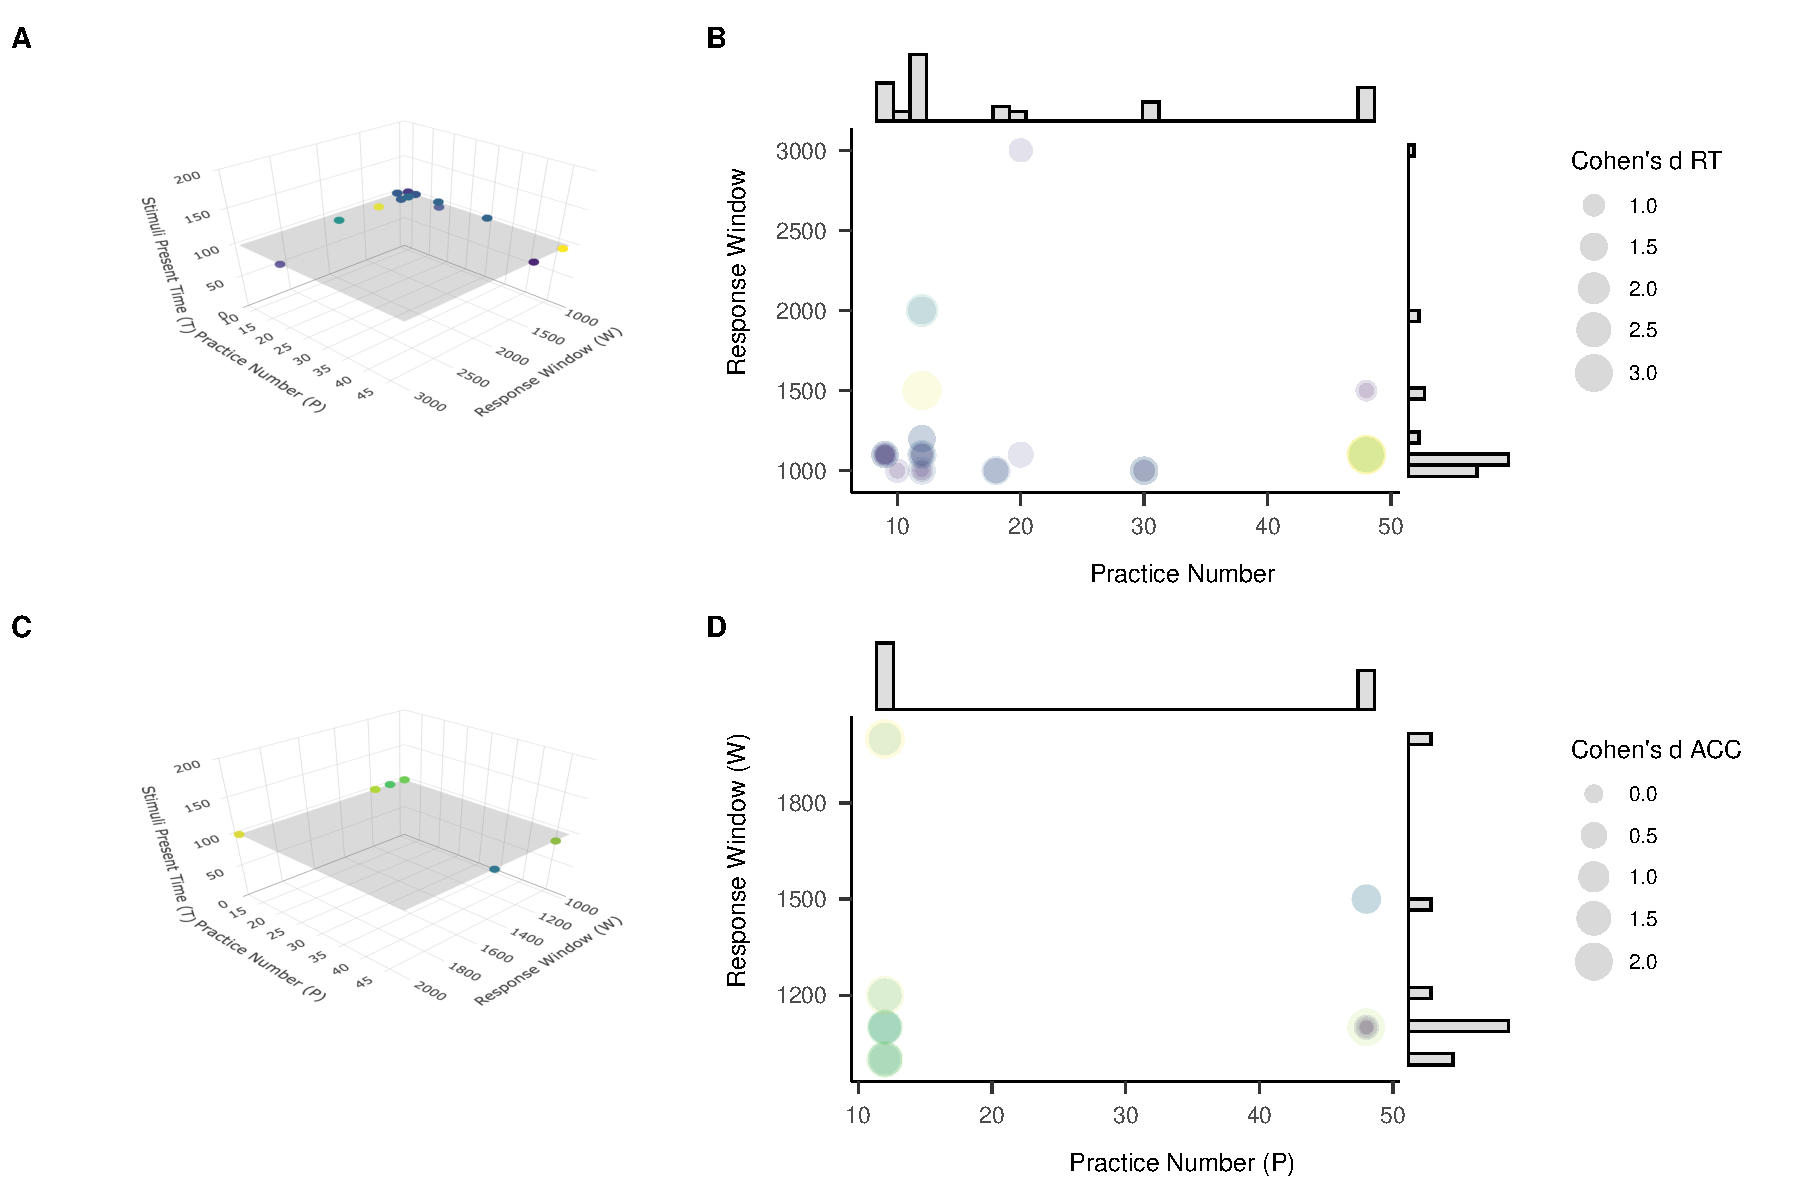
\includegraphics[keepaspectratio]{DesignSpaceSPE_files/figure-latex/fig-figure2-1.pdf}}
\caption{\label{fig:fig-figure2}(A) The scarce distribution of existing experiments with RT data in the three-dimensional design space; (B) Experimental Design Dimensions and Cohen's \(d_{RT}\) of Self-Prioritization Effect; (C) The scarce distribution of existing experiments with ACC data in the three-dimensional design space; (D) Experimental Design Dimensions and Cohen's \(d_{ACC}\) of Self-Prioritization Effect}
\end{figure}

\subsubsection{Discussion}\label{discussion}

Study 1 examined how current available study distributed in the three-dimensional design space and found that most studies that adopted the standard self-matching task are concentrated at a specific value(s) in the space. This lack of exploration of the design space may reflect the current research culture in the field: following previous research settings to obtain statistically significant results.

The findings of Study 1 demonstrated the value of a formal model of experimental design. Once a three-dimensional experimental design space was established, we could view the experimental design from a new angle: how existing studies are closely concentrated in the space, which will not being shown without a three-dimensional space in the first place. A systematical design space, as simple as three-dimensional one, provides a powerful tool for understanding the effect. One consequences of the ignorance of variability in experimental design space is the ignorance of the boundary of the effect we interested in: the boundary of such effect, i.e., the self-prioritization effect in the our case. The scarce distribution in the three-dimensional space also revealed the lack of diversity in experimental task and therefore the generalizability of conclusions of the current studies (Yarkoni, 2022, Behavior and Brain Sciences).

\begin{center}\rule{0.5\linewidth}{0.5pt}\end{center}

\subsection{Study 2: Modelling Experimental Design, Cognitive Process, and Behavioral Outcomes}\label{study-2-modelling-experimental-design-cognitive-process-and-behavioral-outcomes}

\subsection{Method}\label{method-1}

\subsubsection{Research Objective}\label{research-objective-1}

Study 2 aims to formalize the three-dimensional design to bridge experimental design parameters, cognitive processes, and the behavioral outcomes. The verbal description has been described in the Introduction section, below we will present two competing formal models of the verbal model and generate synthesize datasets in the full three-dimensional space, which results in testable competing hypotheses.

\subsubsection{The general model architecture}\label{the-general-model-architecture}

We assume the decision-making process in the self-matching task as an evidence accumulation proccess that involves perception, memory retrieval, and action execution. First, the shape-label association is consolidated in memory and is retrieved during the matching judgment. Second, the visual stimuli are encoded by the visual system and then used for matching judgment. Third, a process that compare sensory information and retrieved association to form the evidence for decision-making (e.g., Myers et al. (2015)). The key assumptions of EAM is that (1) the evidence for decision-making is continuous accumulated with the sensory input and the retrieved association, (2) the decision-making is made when the accumulated evidence reach the decision boundary (Ratcliff, Smith, Brown, and McKoon (2016); Forstmann, Ratcliff, and Wagenmakers (2016); Y. Liu and Hu (2024)). However, under the EAM framework, there are multiple computational models which assumes different cognitive processes and we will consider two of them: the standard drift-diffusion model (DDM) and collapsing boundaries model (ANGLE) (Hawkins, Forstmann, Wagenmakers, Ratcliff, \& Brown, 2015; Leng, Fengler, Shenhav, \& Frank, 2025).

The standard drift-diffusion model as the cognitive process model, which assumes one decision variable (or accumulator), which might be the ``matchness'' between sensory input to the retrieved the shape-label association during the decision-making process Ratcliff and McKoon (2008). And the decision variable was continuous accumulated with the input of visual system (and continue to accumulate after the disappearance of the visual stimuli, \textbf{Citation is needed here}). Also, a decision criteria is set by the participant so that a decision is make when the accumulated evidence reach the criterion and then an action was executed by the motor system. Given the time window allowed for response, participants may actively adjust their criteria (i.e., speed-accuracy trade-off) Bogacz, Brown, Moehlis, Holmes, and Cohen (2010), \textbf{MORE REFs available}.

Under the framework of DDM, the SPE are resulted from self-bias in one of three cognitive processes: the initial bias (\emph{z}), the drift rate (\emph{v}), or the criteria (\emph{a}). First, the self-related stimuli are more likely integrated than other stimuli. Evidence found that self-relevant information are likely to be can encoded more efficiently when the stimuli is uncertain Jie Sui et al. (2012). Second, large volume of studies found that self-related information has advantage in memory Cunningham, Zelazo, Packer, and Van Bavel (2008); Yin and al. (2019). These findings suggest that self-relevant stimuli might enjoy an advantage in drift rate because of the stronger association strength in the self-matching task. However, unlike previous studies that self-relevance served as a cue for immediate strategic adjustment at trial-level (e.g., the cue-target paradigm), in self-matching tasks participants can not predict the label of the next coming trial, so that the initial bias (\emph{z}) is unlikely to be affected in this task. Indeed, previous studies have found that SPE as measured in self-matching task exist for drift rate (\emph{v}). For example Hu et al., (2020) found that the SPE for positive self was primarily driven by the drift rate. Similarly, XXXX \textbf{MORE Refs are needed here}.

Build on these findings, we specify how the change of number of practice trials \emph{P}, stimulus presentation time \emph{T}, and response window \emph{W} will change the drift rat (\emph{v}) and criterion (\emph{a}) in the self-matching task and the SPE.

\paragraph{Number of practice trials, association strength, and drift rate}\label{number-of-practice-trials-association-strength-and-drift-rate}

We assume that the strength of shape-label association is positively related to evidence accumulation rate during decision-making in the self-matching task. And that the strength of association depends on the number of practice trials \emph{P}.

More specifically, we assume increasing \emph{P} increase increases the strength of the shape-label association, which will speed up retrieval of the association during matching judgement, and therefore increase evidence accumulation rate. When \emph{P} = 0 (no practice trials), the strength of association entirely rely on the memory formed at the instruction stage, which may results in a relatively low drift rate \emph{v}. As \emph{P} increases, the strength of association increases and the retrieval efficiency improves, results in higher drift rate \emph{v}. However, our assume comes with one caveat: the number of associations in self-match task is small (usually three) and the shapes and labels are usually simple visual stimuli and familiar words, thus the association strength may saturate soon, even after the instruction stage. Thus, the effect of \emph{P} on drift rate may reach a ceiling soon after a certain number.

We formalize the above assumptions as following: the drift rate \emph{v} increase with \emph{P} increases nonlinearly, with coefficient that slows down and eventually saturate with \emph{P}.

\[v_P = \frac{1}{1 + e^{-k_P(P - P_1)}}\]

\[k_P = k_{min} + \frac{k_{max} - k_{min}}{1 + e^{-\gamma(P - P_0)}}\]

Here the \(k_P\) is the parameter describing the effect of \emph{P} on drift rate, \(k_{min}\) is the minimum value of \(k_P\), \(k_{max}\) is the maximum value of \(k_P\), and \(\gamma\) is the temperature parameter controlling the sensitivity of \(k_P\) to changes in \emph{P}. If \(\gamma\) = 0, XXX, and if \(\gamma\) increase, XXX. In our implementation, we used \(P_0\) to centerize \(k_P(P)\) and \(P_1\) for centerizing \(v_P(P)\).

\paragraph{Presentating time of stimuli, sensory encoding, and drift rate}\label{presentating-time-of-stimuli-sensory-encoding-and-drift-rate}

We assume the sensory input plays an important role in decision-making in the self-matching task. Since visual stimuli in the task are simple (geometric shapes), sensory input is primarily constrained by presentation time \emph{T}. Previous studies show that even after stimuli disappear, individuals' evidence accumulation process can continue for some time Ratcliff and Smith (2004); Zylberberg, Roelfsema, and Sigman (2014). However, the stimulus presentation time may determines the efficiency of evidence accumulation as the continuous visual input is interrupted after stimulus offset. Here we assume that stimulus presentation time \emph{T} determines the sensory input quality and the subsequent evidence accumulation efficiency.

More specifically, when \emph{T} is very short and stimuli are presented subliminally, the sensory input is limited and sensory input can hardly be enough for decision-making. In this case, the overall drift rate \emph{v} is low and the accuracy is low. As \emph{T} increases, sensory input quality increase, which resulted in higher drift rate \emph{v} accordingly. We assume the effect of \emph{T} on overall drift rate has an upper boundary: once the \emph{T} is sufficient for high quality sensory input, additional presenting time will no longer has effect on drift rate \emph{v}.

This assumption is formalize as below:

\[v_T = \frac{1}{1 + e^{-k_T(T - T_0)}}\]

where \(k_T\) is the temperature parameter describing the sensitivity of the effect of \emph{T} on drift rate \emph{v}. In our implementation, we used \(T_0\) to centralize \(v_T\).

\paragraph{The response window, speed-accuracy tradeoff, and decision boundary}\label{the-response-window-speed-accuracy-tradeoff-and-decision-boundary}

We assume that the decision-making in self-matching task, as other forced choice tasks, also regulated by a speed-accuracy trade off. We assume that subjects, who follow the instruction of the experiment and are well-intended, have the motivation to finish the task as fast as accurately as possible under certain time pressure Heitz (2014). The time pressure can be manipulated by the total response window \emph{RW}, which is the sum of stimulus presentation time \emph{T} and response window \emph{W} after the stimulus offset.

\[M \sim f(T + W)\]

We assume that when \emph{M} decreases, time pressure goes high, and participants may prioritize fast response instead of the accuracy. In this case, participants may lower the decision threshold \emph{a}. As \emph{M} increases, the time pressure decreases, participants may increase their decision threshold \emph{a}, and thus increase the accuracy. However, \emph{M}'s effect also saturate when it's longer than accurate response needs.

We formalize the above hypothesis as below:

\[a = \frac{1}{1 + e^{-k_M(M - M_0)}}\]

where \(k_M\) is the temperature parameter for the sensitivity of the effect of \emph{M} on threshold \emph{a}.

\paragraph{The self-prioritization effect in the model}\label{the-self-prioritization-effect-in-the-model}

The above model specifies the relationship between experimental design factors (\emph{P}, \emph{T}, \emph{W}) and the cognitive processes (drift rate \emph{v} and decision threshold \emph{a}). These specifications lay a foundation for the self-prioritization effect, which is the difference in between self-relevant and other-relevant conditions.

We assume experimental design parameters' effect on \emph{v} is modulated by self-relevance of the labels: for the label ``self'', because of its social salience, strength of association increased faster than that of non-self labels, and the sensory input was more efficient, and therefore the \emph{v} for ``self'' is increased faster and reach the ceiling state earlier than that of other conditions. This modulation effect on \emph{v} was formalized as a factor of \(\alpha\).

We also assume that the effect of \emph{M} on \emph{a} is not modulated by self-relevance in our case because participant will not be able to predict the next coming trial is self- or other-relevant trial and it is unrealistic to adjust the threshold upon processing the information based on the standard DDM's model assumption. However, we do aware that the boundary of evidence accumulation may collapse, as assumed by other evidence accumulation model Ratcliff et al. (2016), we adopted the standard DDM here for simplicity and parsimony, and we will consider the collapsing boundary in future model revision.

\paragraph{The Complete Model}\label{the-complete-model}

The effects of these three experimental design dimensions (\emph{P}, \emph{T}, \emph{W}) are not an one-to-one mappings on cognitive processes. Both the number of practice trials \emph{P} and stimulus presentation time \emph{T} affects drift rate \emph{v}.

The parameter \(\alpha\) is a condition factor depending on the current condition (self vs.~stranger), describing the amplification or suppression effect of self-relevance on \emph{v}. Response window \emph{W} modulates decision threshold \emph{a}, determining subjects' decision strategy.

\[v_0 = v_P \cdot v_T \cdot 3\]

\[v = v_0 \cdot (1 + \alpha)\]

\[a_0 = \frac{1}{1 + e^{-k_M(M - M_0)}} \cdot 3\]

\[a =
\begin{cases}
a_0 \cdot (1 + \beta_1), & M > 600 \\
a_0 \cdot (1 + \beta_2), & M \leq 600
\end{cases}
\]

The global scaling factor 3 is retained as an implementation-level scaling constant to keep simulated drift and boundary magnitudes in a numerically stable and interpretable range for downstream simulation and visualization.

This model mathematically quantifies the interaction between these factors, providing a tool for quantitatively assessing changes in the self-prioritization effect under different experimental conditions. This approach not only supports establishing a quantitative theoretical framework but also helps deeply understand key mechanisms in cognitive decision-making processes.

\subsubsection{Model specification and implementation}\label{model-specification-and-implementation}

Python 3.11.5 was used to generate data. This study randomly generated simulated data for 300, 000 subjects (0.26\% of the full space), with each subject completing 260 trials. Each subject's experimental design combination was randomly sampled from the three-dimensional design space \emph{P}, stimulus presentation time \emph{T}, and response window \emph{W}. In implementation, these parameters are sampled as discrete integers (upper bound excluded, consistent with \texttt{np.random.randint}):

\[P \in \{0, 1, \dots, 149\}\]
\[T \in \{10, 11, \dots, 599\}\]
\[W \in \{200, 201, \dots, 1499\}\]

Based on the formulas in the theoretical model, each subject's experimental design combination (\emph{P}, \emph{T}, \emph{W}) yields the base drift rate \(v_0\) and base decision threshold \(a_0\) after calculation. Decision threshold \emph{a} varies at the subject level, randomly drawn from normal distribution \(N(a_0, a_0 \cdot A_{CV})\) (implemented with \(A_{CV}=0.15\)). Drift rate \emph{v} varies at the trial level, randomly drawn from normal distribution \(N(v_0, 1)\). Starting point \emph{z} is fixed at \emph{a}/2, and non-decision time \(t_0\) is fixed at 0.2 s.

Evidence accumulation adopts a sampling interval of 1 ms (minimum time step), with each sample's noise drawn from normal distribution \(N(0, 1)\), following the stochastic differential equation:

\[dx = v\Delta t + \varepsilon\sqrt{\Delta t}\]

The stopping condition for the evidence accumulation process follows the implemented rule: maximum allowed decision time is

\[t_{max} = (W + T - t_0) \cdot 0.001 + 0.001\]

where \emph{T} and \emph{W} are in ms and \(t_0\) is in s. A trial is recorded as valid only when evidence reaches a boundary in time (\texttt{response\ \textgreater{}\ 0} and \texttt{decision\textbackslash{}\_time\ \textless{}\ t\_\{max\}}). If this criterion is not met, the trial is invalid and no response is recorded.

For outcome coding, the simulator directly outputs boundary-hit response (\texttt{response}) rather than a direct task-level correctness variable. In this Study 2 pipeline, simulation and downstream behavioral summaries focus on match-trial dynamics; therefore, ACC interpretation is based on an explicit post-simulation mapping rule from latent boundary-hit outcomes to correctness coding.

\subsubsection{Data Analysis}\label{data-analysis-1}

R was used for analyzing the synthetic data. We focused on the behavioral outcomes and standardized effect size (Cohen' \emph{d}). Specifically, the study calculated the effect size of the self-prioritization effect at the subject level for RT and ACC, where \emph{n} in the formula is the number of trials in each condition (citation needed).

\[Cohen's\ d = \frac{M_1 - M_2}{S_{pool}}\]

\[S_{pool} = \sqrt{\frac{(n_1 - 1) \cdot \sigma_1^2 + (n_2 - 1) \cdot \sigma_2^2}{n_1 + n_2 - 2}}\]

To keep the direction of the effect size, the effect size for the RT was based on \(RT_{stranger} - RT_{self}\), and ACC on \(ACC_{stranger} - ACC_{self}\). Larger effect sizes indicate larger self-prioritization effects. Visualization was conducted using 3D space and contour plots that fitted with Gaussian additive model (citation needed).

\subsubsection{Results}\label{results-1}

The synthetic data based on our model revealed a clear pattern for the effect of experimental design factor on cognitive processes and the downstreaming behaviorual outcomes.

For RT, Cohen's \(d_{RT}\) was mainly affected by response window \emph{W} and stimulus presentation time \emph{T} (Figure 4). Consistent with model assumptions, as \emph{W} and \emph{T} increased, the self-prioritization effect gradually strengthened. As shown in Figure 4 (bottom left), the effect size of the self-prioritization effect approached 0 under conditions of short \emph{W} (200-600 ms) and short \emph{T} (0-200 ms). This means that when time is extremely limited, self-related information's, as other-related information, is insufficiently processed and there is no self-prioritization effect. Also, we found that, cross the entire parameter space, the number of practice trials \emph{P} had no effect on Cohen's \(d_{RT}\). This result indicates that SPE on RT is primarily shaped by experimental design factors that related to time, but not so much the number of practice trials. This is not surprising given that the standard self-matching task is relatively simple and practices may not enhance the memnomic association between shapes and labels.

\[ Insert Figure 4 here, Figure 4. Synthetic data for SPE in RTs (Cohen's *d*, A-D) and Accuracy (E-H), (A) 3-D screenshot; (B) 2d contour plots with GAM smoothing, *P* as the x-axis and *W* as y-axix; (C) W: x-axis, T: Y-axis; (D), P: x-axis; T:Y-axis ; (E): 3-D screenshot of ACC; (F) 2d contour plot with GAM smoothing; (G) ...; (H) ...\]

For ACC, Cohen's \(d_{ACC}\) was mainly affected by response window \emph{W} and stimulus presentation time \emph{T} (Figure 5). As shown in Figure 5 (bottom left), the effect size of the self-prioritization effect approached 0 or even showed effect reversal under conditions of short \emph{W} (200-400 ms) and short \emph{T} (0-150 ms). When \emph{T} was 0-130 ms, as \emph{W} increased, the self-prioritization effect gradually strengthened. When \emph{W} was 200-400 ms, as \emph{T} increased, the self-prioritization effect first strengthened then weakened. This indicates that as time pressure decreases, the effect size of the self-prioritization effect on accuracy gradually shows ceiling effects. In the range of \emph{W} \textgreater{} 400 ms, \emph{T} \textgreater{} 130 ms, the low values of Cohen's \(d_{ACC}\) can also illustrate this. Similar to Cohen's \(d_{RT}\), as shown in Figure 5 (right), the number of practice trials \emph{P} did not show significant regulatory effects across the entire parameter space.

\subsubsection{Discussion}\label{discussion-1}

Study 2 constructed a three-dimensional experimental design space for the self-prioritization effect under the self-matching task, achieved systematic simulation of ``experimental design-cognitive process-data results,'' and quantified the dynamic change characteristics of the self-prioritization effect with different experimental design dimensions according to model assumptions.

By incorporating experimental design into computational models, this study further expanded the scope of computational models, truly making experimental design the foundation of theoretical construction. This approach effectively connects theory-driven and data-driven research paths, providing a new modeling paradigm Griffiths and Blei (2010). In the model construction process, for operational and complexity trade-offs, experimental design parameter dimensions were limited to three easily quantifiable variables. Although such simplification may lead to some high-order interaction effects being ignored, it effectively balances model explanatory power and computational feasibility Sun (2008).

The simulation results of this study not only provide a new explanatory perspective for understanding the self-prioritization effect but also point out key verification paths for subsequent experimental research. Specifically, this study is the first to point out that the self-prioritization effect has boundaries, helping resolve current controversies about the self-prioritization effect J. Sui and Humphreys (2015); Golubickis and Macrae (2023). Although previous researchers generally believed that the self-prioritization effect has boundaries, the boundary conditions were not clear. The model of this study points out that the critical values of W and T mark the boundary of the self-prioritization effect from resource competition to stable expression. In the range of W = 200-600 ms and T = 0-150 ms, the effect size of the self-prioritization effect shows high sensitivity to small parameter changes, providing a ``strong test region'' for empirical verification Platt (1964). If empirical data cannot reproduce the effect size gradient in this region, the current model assumptions may need revision. The finding that P has no significant influence on the self-prioritization effect across the full parameter space conflicts with existing research---self-related information processing in matching conditions is more easily enhanced by practice Reuther and Chakravarthi (2017). If subsequent empirical research observes empirical dependence of the self-prioritization effect at P \textgreater{} 100, adaptive gain regulation mechanisms need to be introduced to improve the current model.

In summary, Study 2 not only explored the boundary conditions of the self-prioritization effect through formal modeling and simulation system of experimental design but also provided a new theoretical perspective for understanding self-related information processing mechanisms, while demonstrating a generalizable theoretical construction path based on experimental design space. This methodological framework has strong generality and can be extended to modeling and verification work of other cognitive phenomena in the future.

\begin{center}\rule{0.5\linewidth}{0.5pt}\end{center}

\subsection{Study 3: Empirical Analysis}\label{study-3-empirical-analysis}

\subsection{Method}\label{method-2}

\subsubsection{Research Objective}\label{research-objective-2}

Based on the results of Study 2, Study 3 systematically samples in the design space by manipulating experimental design dimensions (such as number of practice trials, stimulus presentation time, and response window) to form specific experimental designs and conduct data collection, testing the predictive effects of the theory from Study 2. By comparing simulated data and empirical data, the theoretical model is tested, providing important feedback for subsequent model and theoretical framework optimization. Specifically, simulated data, based on theoretical assumptions, reflect potential changes in cognitive mechanisms under different experimental conditions, while empirical data are obtained from actual subjects to verify these theoretical assumptions. By ensuring consistent parameter settings for the same experimental conditions between simulated and empirical data, data comparability is guaranteed. The research focus is on analyzing the effect size differences and parameter differences between simulated data and empirical data under different experimental conditions. This difference helps more deeply understand the relationship between theoretical assumptions and actual cognitive mechanisms and provides important guidance for further optimizing the theoretical framework and generative model.

\subsubsection{Research Design}\label{research-design}

{[}TABLE: Figure 6 - Experimental Design Parameter Selection Visualization{]}

The experimental condition settings in this study are not uniform sampling or completely symmetric design, following three considerations: First, based on the simulation results in Study 2, as shown in Figure 6, parameter combinations with simulated effect sizes at critical transition regions or boundaries are preferentially selected, ensuring experimental conditions cover the most diagnostically significant task intervals predicted by the model; second, constructing a task gradient from extreme cognitive resource limitation to resource saturation, systematically examining the change patterns of the self-prioritization effect under different conditions; third, manipulating one experimental design dimension while keeping other parameters constant to identify the independent influence of the corresponding cognitive process on behavioral results.

Under this design framework, this study hypothesizes that the effect size of the self-prioritization effect shows systematic changes across experimental conditions (H1). The cognitive process changes caused by parameter manipulation in empirical experiments will be consistent with the trend of DDM parameter changes in theoretical simulation (H2). Specifically, the following 6 experimental designs are included:

\textbf{Design 1: Extreme Case (\emph{P} = 0 trials, \emph{T} = 30 ms, \emph{W} = 300 ms)}

This design is at the lowest resource boundary of the experimental design space, intended to test whether the self-prioritization effect is observable at the behavioral level under the extreme situation of insufficient perceptual information, unconsolidated memory, and almost no response margin.

In the perceptual stage, the 30 ms stimulus presentation time allows subjects to obtain only blurry, fragmented visual features, with low signal-to-noise ratio. The incompleteness of perceptual input leads to lack of clear direction in the initial evidence accumulation. In the memory stage, since the number of practice trials is 0, subjects must rely on initial encoding that has not yet solidified for matching. Under high load tasks, memory retrieval is susceptible to interference, and retrieval efficiency and accuracy are at low levels. In the decision stage, the 300 ms response window approaches the shortest possible boundary for human judgment response. Under such extreme time pressure, subjects cannot fully accumulate evidence and can only make responses based on momentary impulses.

Under this highly constrained triple-task setting, although self-related stimuli theoretically have the potential to promote evidence integration, their compensatory role cannot be fully exerted under extreme cognitive resource insufficiency, and floor effects will be exhibited. It is predicted that under this design, the self-prioritization effect cannot be observed at the behavioral level, and effect sizes on both RT and ACC approach 0.

\textbf{Design 2: Extended Response Window (\emph{P} = 0 trials, \emph{T} = 30 ms, \emph{W} = 600 ms)}

This design retains perceptual limitations and no practice trials while extending the response window to 600 ms, intended to test whether extending the response window helps enhance the self-prioritization effect, i.e., whether the self-prioritization effect can be initially observed at the behavioral level under limited input information by merely adjusting decision strategy.

In perceptual and memory stages, it is the same as Design 1. However, in the decision stage, the increase in response window eases time pressure, and subjects have greater strategic flexibility to regulate decision thresholds.

Under this situation, although perceptual and memory processing resources remain limited, the processing advantages of self-related information have initially appeared in behavioral performance. Subjects may preferentially rely on self-related cues based on limited evidence, thereby achieving more stable judgment performance. Therefore, it is predicted that the effect size of the self-prioritization effect on RT and ACC will increase compared to Design 1, showing initial behavioral differentiation. When response window increases from Design 1 (\emph{W} = 300 ms) to Design 2 (\emph{W} = 600 ms), the change trend of empirical data DDM parameter \emph{a} is consistent with \emph{a} based on Study 2 simulation data, verifying the theoretical expectation of regulating decision strategy in cognitive mechanisms.

\textbf{Design 3a: Increased Number of Practice Trials (\emph{P} = 120 trials, \emph{T} = 30 ms, \emph{W} = 600 ms)}

This design increases the number of practice trials to 120 while keeping other settings consistent with Design 2, intended to test whether improving memory retrieval efficiency helps enhance the behavioral performance of the self-prioritization effect.

The key difference from Design 2 lies in the memory stage. The increase in the number of practice trials causes subjects to have experienced the shape-label pairing task multiple times before the formal experiment, making the memory representation of shape-label associations more consolidated, and the retrieval process faster and more resistant to interference.

Based on the simulation results in Study 2, the improvement in memory may have equal effects on the retrieval efficiency of self and stranger conditions, which may not be sufficient to significantly widen the gap between the two at the behavioral level. Therefore, it is predicted that the effect size of the self-prioritization effect on RT and ACC will have small difference from Design 2. When the number of practice trials increases from Design 2 (P = 0) to Design 3a (P = 120), the change trend of drift rate difference \(v_{self} - v_{stranger}\) in empirical data is consistent with that in simulation data based on Study 2, verifying the theoretical expectation of changes in memory retrieval efficiency in cognitive mechanisms.

\textbf{Design 4a: Extended Stimulus Presentation Time (\emph{P} = 120 trials, \emph{T} = 80 ms, \emph{W} = 600 ms)}

This design extends stimulus presentation time to 80 ms while keeping other parameter settings unchanged, intended to test whether improving perceptual input quality helps enhance the behavioral performance of the self-prioritization effect.

In the perceptual stage, stimulus presentation time increases from 30 ms to 80 ms, providing subjects with more time to extract stimulus features. Visual input is more complete, signal-to-noise ratio improves, the clarity and stability of perceptual evidence improve, and the directionality and efficiency of evidence accumulation in the initial stage improve.

Under this design, subjects can quickly and accurately retrieve established self-associations, exerting the integration advantages of self-related information. Therefore, it is predicted that the effect sizes of the self-prioritization effect on RT and ACC will significantly increase compared to Design 3a. When stimulus presentation time increases from Design 3a (\emph{T} = 30 ms) to Design 4a (\emph{T} = 80 ms), the difference in empirical data DDM parameter \emph{v} (\(v_{self} - v_{stranger}\)) is consistent with the change trend of \(v_{self} - v_{stranger}\) in simulation data based on Study 2, and DDM parameter \emph{a} is consistent with the change trend of \emph{a} based on Study 2 simulation data, verifying the theoretical expectation of changes in perceptual input quality in cognitive mechanisms.

Note that we conducted two additional studies to increase the response window \emph{W} so that the condition is easier compared to Design 3a and Design 4a. Specifically, Design 3b (\emph{P} = 120 trials, \emph{T} = 30 ms, \emph{W} = 800 ms) and Design 4b (\emph{P} = 120 trials, \emph{T} = 80 ms, \emph{W} = 800 ms).

\textbf{Design 5: Baseline (\emph{P} = 8 trials, \emph{T} = 100 ms, \emph{W} = 1100 ms)}

This design uses commonly used task parameter settings in the self-matching paradigm (P = 8 trials, i.e., 2 practice trials per label \(\times\) shape, consistent with P = 12 in the standard task), serving as a control baseline under standard task conditions to evaluate the relative changes in self-prioritization effect performance under various experimental designs.

In the perceptual stage, the 100 ms stimulus presentation time provides subjects with sufficient visual input time. Stimulus features can be fully extracted, perceptual quality is high, and signal-to-noise ratio is good, contributing to generating stable perceptual evidence. In the memory stage, the number of practice trials is 8, the association relationship has been initially established but not yet fully automated, memory retrieval is relatively effective but still has some fluctuations. In the decision stage, the 1100 ms response window provides sufficient time resources, subjects can flexibly regulate decision thresholds, trade off between speed and accuracy, and improve response stability.

This design provides a relatively ideal environment for the processing advantages of self-related information to be exerted. Individuals can quickly retrieve self-association content and make responses with sufficient evidence support. Therefore, it is predicted that under this design, the self-prioritization effect will be stably exhibited on both RT and ACC dimensions.

\textbf{Design 6: Saturation Case (\emph{P} = 120 trials, \emph{T} = 500 ms, \emph{W} = 1500 ms)}

This design sets the maximum values of experimental design dimension values (\emph{P}, \emph{T}, \emph{W}) in the theoretical model, constructing a processing environment with the most sufficient cognitive resources, intended to test whether the behavioral performance of the self-prioritization effect enhances when perception is most complete, memory is most solid, and time is most abundant.

In the perceptual stage, the 500 ms stimulus presentation time is far above the perceptual saturation threshold, ensuring subjects fully acquire stimulus features. Visual input is almost lossless, signal-to-noise ratio is extremely high, and perceptual evidence is highly clear. In the memory stage, 120 practice trials make the shape-label association reach a highly automated level, the retrieval process is fast, stable, and almost unaffected by interference, further improving evidence accumulation efficiency. In the decision stage, the 1500 ms response window provides subjects with sufficient strategic flexibility, prompting individuals to complete judgments under higher accuracy requirements.

Under this optimal configuration of multiple resources, the integration advantages of self-related information are maximally released. Individuals can not only quickly identify self-related visual features but also efficiently retrieve association information and make accurate decisions after sufficient evidence accumulation. Therefore, it is predicted that the effect size of the self-prioritization effect on RT will significantly increase. However, on the accuracy dimension, as overall accuracy approaches the ceiling, ceiling effects may occur, causing the difference between self and stranger conditions to relatively narrow, and the effect size to instead decrease.

\subsubsection{Participants}\label{participants}

A total of 8 groups of subjects were recruited. All subjects were healthy adults, right-handed, with normal or corrected-to-normal vision, and no known neurological or psychiatric disorders. All subjects received monetary compensation after the experiment.

\begin{table}[tbp]

\begin{center}
\begin{threeparttable}

\caption{\label{tab:tbl-demographics}Demographic Information and Trial Counts by Experimental Design}

\begin{tabular}{llllll}
\toprule
DesignId & \multicolumn{1}{c}{Exp Design (P, T, W)} & \multicolumn{1}{c}{N (females)} & \multicolumn{1}{c}{Age (M ± SD)} & \multicolumn{1}{c}{$Trials_{total}$} & \multicolumn{1}{c}{$Trial_{valid}$}\\
\midrule
D1 & P=0, T=30, W=300 & 11 (8) & 23.1 ± 1.2 & 5720 & 1625\\
D2 & P=0, T=30, W=600 & 12 (9) & 22.6 ± 2.1 & 6240 & 2868\\
D3a & P=120, T=30, W=600 & 10 (7) & 22.7 ± 2.1 & 5200 & 3222\\
D3b & P=120, T=30, W=800 & 11 (11) & 22.9 ± 1.5 & 5720 & 3478\\
D4a & P=120, T=80, W=600 & 12 (12) & 21.8 ± 1.6 & 6240 & 4786\\
D4b & P=120, T=80, W=800 & 11 (9) & 22.7 ± 1.6 & 5720 & 4834\\
D5 & P=8, T=100, W=1100 & 11 (7) & 23.3 ± 1.2 & 5720 & 5089\\
D6 & P=120, T=500, W=1500 & 10 (10) & 22.1 ± 2 & 5200 & 4927\\
\bottomrule
\end{tabular}

\end{threeparttable}
\end{center}

\end{table}

In addition to real experimental data, this study generated simulated data under the same experimental designs using the model from Study 2, for comparison with real data. There were 8 subjects under each design, and each subject completed 260 matching trials.

\subsubsection{Materials}\label{materials}

The experimental program was written using Matlab 2022b software's Psychtoolbox 3.0 toolbox Brainard (1997); Kleiner, Brainard, and Pelli (2007). Visual stimuli were presented on a Dell P1130 CRT monitor with a screen resolution of 1024 \(\times\) 960 and a refresh rate of 85 Hz. Subjects were positioned 70 cm from the screen. The shapes included squares and circles (size 3.8\(^\circ\) \(\times\) 3.8\(^\circ\)), presented above the central fixation point (0.0.8\(^\circ\) \(\times\) 0.8\(^\circ\)) on the screen, while the labels ``Self'' and ``Stranger'' (size 3.1\(^\circ\) \(\times\) 1.6\(^\circ\)) were displayed below the fixation point. The distance between the center of the shape or label and the fixation cross was 3.5\(^\circ\). All stimuli were white ({[}255, 255, 255{]}) on a grey background ({[}128, 128, 128{]}).

Different from the standard paradigm, some experimental designs in this study used shorter stimulus presentation times. To effectively control perceptual interference, this experiment used mask stimuli. To reduce confounding variables, all designs used mask stimuli (the specific effects of masked vs.~unmasked stimuli can be seen in the pre-experiment results in Appendix B). The mask stimuli consisted of images of the same size as the labels ``Self'' and ``Stranger,'' processed using Adobe Photoshop 2025's Scramble Filter with Tile Width and Tile Height both set to 10 pixels to scramble their original structure and produce visual noise, thereby interfering with subjects' processing of target stimuli. The mask stimulus display time was fixed at 150 ms to effectively prevent subjects from further processing label information, thereby reducing memory and attention biases.

\subsubsection{Procedure}\label{procedure}

The experiment was conducted in a soundproofed laboratory, with subjects seated directly in front of the screen, ensuring eyes were approximately 70 cm from the screen. The experiment was expected to take approximately 20 minutes. Before the experiment began, the experimenter first guided subjects to read the ``Informed Consent Form for Participation'' and ``Informed Consent Form for Data Publication.'' After obtaining subject consent, the experiment officially began.

Referring to Jie Sui et al. (2012), the first stage of the experiment was the association stage. In this stage, the screen presented instructions requiring subjects to associate the two labels ``Self'' and ``Stranger'' with the two geometric shapes ``Circle'' and ``Square.'' For example, subjects were instructed to associate ``Self'' with ``Circle'' and ``Stranger'' with ``Square.'' The association relationship was presented for 60 s. In this stage, not specific shapes but the text form of label-shape association was presented.

After subjects mastered the association instructions, they entered the matching stage, with the procedure shown in Figure 7. According to different groups, subjects in each group were assigned different numbers of practice trials \emph{P}, stimulus presentation time \emph{T}, and response window \emph{W}. Each trial started with a central fixation point lasting 500 ms. Then the shape-label pair was presented for \emph{T} ms, followed by a 150 ms mask stimulus, then a blank screen for W - 150 ms. Subjects needed to quickly and accurately judge whether the shape-label pair presented on the screen was consistent with the previously learned association within the designated response window. If the shape-label pair was consistent with the initial association, subjects pressed the F key; if inconsistent, they pressed the J key. After the judgment, feedback appeared on the screen for 500 ms, displaying ``Correct'' or ``Error'' based on subjects' response. If RT was within 150 ms, feedback was ``Too Fast''; if the response was not completed within the specified window, feedback was ``Too Slow.'' The association relationship and key assignment were balanced between subjects. After completing practice trials, formal experimental trials began, with the same procedure as the practice stage, the only difference being that no immediate feedback was provided during formal experiments, only displaying ACC and mean RT at the end of each block.

The formal experiment consisted of 520 trials divided into 10 blocks, with self-matching, self-mismatching, stranger-matching, and stranger-mismatching stimuli presented pseudo-randomly in equal proportions. Thus, the number of trials for each condition (self-matching, self-mismatching, stranger-matching, stranger-mismatching) was 130.

{[}FIGURE: Figure 7 - Self-Matching Task Flowchart{]}

\subsubsection{Data Analysis}\label{data-analysis-2}

The purpose of this study was to examine the changes in the self-prioritization effect under different experimental designs by adjusting key parameters in experimental design (number of practice trials, stimulus presentation time, and response window), and to test the influence of experimental manipulation on the self-prioritization effect by comparing simulated and empirical data. Data analysis was based on trials where subjects made responses in matching conditions.

Due to the relatively small sample size, this study used the robust statistical method bootstrap for analysis to obtain robust effect size distributions of the self-prioritization effect under each experimental design. For each subject's data, 5000 resamples were conducted. In each iteration, the subject's data under the current design were first grouped by label (Self/Stranger), then independent resampling was conducted on the response data of the two groups. Based on the data from each sample, means and standard deviations were calculated, and Cohen's \emph{d} was calculated accordingly. The effect size calculation method remained consistent with Study 2 to ensure comparability across studies. Each subject under each experimental design would produce a distribution containing 5000 Cohen's d values, used to describe the individual effect size estimates of the self-prioritization effect under that design. At the group level, effect size distributions of all subjects were summarized to form the behavioral performance of the self-prioritization effect under different designs. Furthermore, to verify the accuracy of model predictions, the Cohen's \emph{d} under each experimental design in empirical data was further compared with predicted values in simulated data from Study 2, to evaluate the predictive power of the theoretical model for the change pattern of the self-prioritization effect under different experimental design dimensions.

To deeply explore subjects' psychological processes under different experimental designs, this study compared simulated data with empirical data. For simulated data, RT and keypress response data were generated by setting the same experimental parameters \emph{P}, \emph{T}, \emph{W} as empirical data. DDM parameters \emph{v} and \emph{a} were obtained through theoretical formulas during data generation. For empirical data, fast-dm-30 (Voss, Nagler, \& Lerche, 2015) was used to conduct DDM modeling on individual subjects' RT and keypress responses, using maximum likelihood estimation (MLE) to estimate drift rate v and decision threshold \emph{a}. During estimation, drift rate \emph{v} varied according to experimental labels, decision threshold \emph{a} was optimized as a free parameter, and non-decision time \(t_0\), starting point variability \(s_z\), and other parameters were kept consistent with the theoretical model to control potential interference from these factors. Bootstrap was conducted using each group's parameter values as a set, and further analysis was conducted according to Hypothesis 2. By comparing the fitting results of simulated data and empirical data under various experimental designs, the effectiveness of the experimental design and model in capturing subjects' psychological processes could be evaluated, and the potential mechanisms of the self-prioritization effect under different experimental designs could be further revealed.

When judging whether the self-prioritization effect under a certain experimental design is significant, the study checked whether its bootstrap 95\% CI included 0. If the bootstrap 95\% CI includes 0, then there is no significant effect; otherwise, it is considered significant. Using whether bootstrap 95\% CIs overlap was adopted as the criterion for judging statistical significance Cumming and Finch (2005). Similarly, if the bootstrap 95\% CIs of two conditions overlap, then there is no significant difference between them; otherwise, there is a statistically significant difference.

\subsubsection{Results}\label{results-2}

To systematically examine the behavioral performance of the self-prioritization effect under different experimental design dimensions, this study calculated and plotted Cohen's \emph{d} and its distribution for both RT and ACC indicators.

As shown in Figure 7 (left), on RT, the distribution of Cohen's \(d_{RT}\) for the self-prioritization effect under experimental designs with W \(\leq\) 600 ms showed some fluctuations but did not show obvious systematic change trends. The effect size distributions under experimental designs with W \(\leq\) 600 ms were all concentrated between -1 and 1, with highly overlapping distributions between self and stranger conditions, and the difference was not significant. This indicates that under these settings, the behavioral performance of the self-prioritization effect on RT is very limited. This result shows that although T and P were manipulated in these four experimental designs, as long as W is at a short level, the performance of the self-prioritization effect on RT is always constrained. In other words, W may be a key factor limiting the performance of the self-prioritization effect on RT. Even with increased stimulus presentation time or practice trials, without sufficient time for evidence accumulation, stable self-processing advantages are still difficult to form. Relatively, only under baseline conditions (\emph{P} = 8, \emph{T} = 100 ms, \emph{W} = 1100 ms) and saturation conditions (\emph{P} = 120, \emph{T} = 500 ms, \emph{W} = 1500 ms) did the RT effect size of the self-prioritization effect show obvious enhancement. As can be seen in the figure, under these two experimental designs, Cohen's \(d_{RT}\) shifted rightward, and the RT distribution of self condition was generally left of stranger condition, indicating that with sufficient RT, self-related information processing advantages were able to manifest.

Further comparing simulated data and empirical data, as shown in Figure 8 (top), the model overall captured the main effect patterns of RT and Cohen's \(d_{RT}\) under various experimental designs relatively well. From Design 1 to Design 5, simulated data and empirical observations were highly consistent in effect direction, with self condition RT generally faster than stranger condition. The effect sizes also showed good consistency, indicating that the model has certain predictive power for decision-making process changes caused by response window, number of practice trials, and stimulus presentation time variables. However, under Design 6 (\emph{P} = 120, \emph{T} = 500 ms, \emph{W} = 1500 ms), the simulated data showed a ceiling effect, while the empirical data showed continued growth. This discrepancy indicates that the model may have certain limitations under conditions of very sufficient resources.

\begin{table}[tbp]

\begin{center}
\begin{threeparttable}

\caption{\label{tab:tbl-design-effect-sizes}Design Parameters and Effect Sizes: Model Predictions vs Empirical Data}

\begin{tabular}{llllllll}
\toprule
Design & \multicolumn{1}{c}{P} & \multicolumn{1}{c}{T} & \multicolumn{1}{c}{W} & \multicolumn{1}{c}{$d_{RT,pred}$} & \multicolumn{1}{c}{$d_{RT}$} & \multicolumn{1}{c}{$d_{ACC,pred}$} & \multicolumn{1}{c}{$d_{ACC}$}\\
\midrule
D1 & 0 & 30 & 300 & 0.03 & 0.00 & 0.22 & 0.01\\
D2 & 0 & 30 & 600 & 0.25 & -0.01 & 0.87 & 0.29\\
D3a & 120 & 30 & 600 & 0.35 & -0.04 & 0.91 & 0.21\\
D3b & 120 & 30 & 800 & 0.43 & 0.04 & 0.93 & 0.48\\
D4a & 120 & 80 & 600 & 0.51 & 0.18 & 0.87 & 0.50\\
D4b & 120 & 80 & 800 & 0.63 & 0.23 & 0.81 & 0.36\\
D5 & 8 & 100 & 1100 & 0.75 & 0.35 & 0.80 & 0.42\\
D6 & 120 & 500 & 1500 & 2.20 & 0.31 & 0.26 & 0.09\\
\bottomrule
\end{tabular}

\end{threeparttable}
\end{center}

\end{table}

\begin{table}[tbp]

\begin{center}
\begin{threeparttable}

\caption{\label{tab:tbl-ddm-parameters}DDM Parameters: Model Predictions vs Empirical Data}

\begin{tabular}{llllllllllll}
\toprule
Design & \multicolumn{1}{c}{P} & \multicolumn{1}{c}{T} & \multicolumn{1}{c}{W} & \multicolumn{1}{c}{$v_{self,pred}$} & \multicolumn{1}{c}{$v_{self}$} & \multicolumn{1}{c}{$v_{str,pred}$} & \multicolumn{1}{c}{$v_{str}$} & \multicolumn{1}{c}{$v_{diff,pred}$} & \multicolumn{1}{c}{$v_{diff}$} & \multicolumn{1}{c}{$a_{pred}$} & \multicolumn{1}{c}{$a$}\\
\midrule
D1 & 0 & 30 & 300 & 2.15 & 1.84 & 0.52 & 1.86 & 1.64 & -0.02 & 0.23 & 0.57\\
D2 & 0 & 30 & 600 & 2.52 & 0.68 & 0.76 & 0.22 & 1.76 & 0.46 & 2.15 & 0.94\\
D3a & 120 & 30 & 600 & 3.01 & 0.60 & 0.94 & -0.06 & 2.07 & 0.65 & 2.16 & 0.92\\
D3b & 120 & 30 & 800 & 3.12 & 1.69 & 1.17 & 0.66 & 1.95 & 1.03 & 3.30 & 1.48\\
D4a & 120 & 80 & 600 & 3.57 & 1.23 & 1.20 & 0.29 & 2.37 & 0.94 & 2.45 & 1.36\\
D4b & 120 & 80 & 800 & 3.62 & 1.79 & 1.38 & 1.14 & 2.24 & 0.66 & 3.38 & 1.80\\
D5 & 8 & 100 & 1100 & 3.23 & 1.67 & 1.16 & 0.73 & 2.07 & 0.94 & 3.59 & 1.82\\
D6 & 120 & 500 & 1500 & 7.29 & 2.54 & 1.99 & 2.07 & 5.30 & 0.48 & 3.60 & 3.60\\
\bottomrule
\end{tabular}

\end{threeparttable}
\end{center}

\end{table}

{[}Add comparison figures between simulated and empirical data{]}

{[}FIGURES: Figures 7-10 - Empirical Data Bootstrap Results and Comparison with Simulated Data{]}

To examine whether increasing \emph{T} can stably promote the behavioral performance of the self-prioritization effect when \emph{P} and \emph{W} are both at sufficient levels, Empirical Study selected two key experimental designs in the space: Design 3b (\emph{P} = 120, \emph{T} = 30 ms, \emph{W} = 800 ms) and Design 4b (\emph{P} = 120, \emph{T} = 80 ms, \emph{W} = 800 ms). \emph{T}'s increase had different effects on the behavioral performance of the self-prioritization effect on RT and ACC.

On RT, as shown in Figure 11 (left), Study 4 results showed that extending response window had a significant promoting effect on the effect size of the self-prioritization effect. Compared with Design 3 and Design 4 in Study 3 with the same T and P settings but shorter response windows (W = 600 ms), the Cohen's \(d_{RT}\) under the two designs in the extended designs (W = 800 ms) showed overall rightward shift, and the effect size distribution was more concentrated, indicating that the wider window provided subjects with more sufficient evidence accumulation opportunities, thereby enhancing the processing advantage of self condition. However, further comparison between Design 3b and Design 4b showed that T's increase had relatively limited influence on the self-prioritization effect on RT, with their Cohen's \(d_{RT}\) distributions highly overlapping and the overall trend not showing systematic enhancement. This result suggests that under sufficient practice trials and response time, further increasing stimulus presentation time does not have a decisive contribution to the behavioral performance of the self-prioritization effect on the speed dimension, indicating that perceptual influence on speed output may have an upper limit or strategic compensation mechanism intervention.

On ACC, as shown in Figure 11 (right), the two designs in the extended designs (W = 800 ms) compared with corresponding Design 3 and Design 4 in Study 3 (W = 600 ms) showed overall higher concentration and stability in Cohen's \(d_{ACC}\) distribution, suggesting that a wider response window helps enhance the behavioral performance of the self-prioritization effect on ACC. However, contrary to intuition, when T increased from 30 ms to 80 ms, Cohen's \(d_{ACC}\) actually decreased. Further observation of the behavioral distributions of self and stranger conditions showed that this weakening mainly came from the improvement in accuracy in the stranger condition, not the decline in self condition. This result suggests that the enhancement of perceptual input not only optimizes self-information processing but may also improve perceptual integration efficiency for stranger information, thereby weakening the relative advantage of the self-prioritization effect.

As shown in Figure 12, simulated data and empirical observations were highly consistent in effect direction, with self condition RT generally faster than stranger condition; effect size differences were small, and model predictions were relatively accurate.

Further comparing the change trend of drift rate difference \(v_{self} - v_{stranger}\) between simulated data and empirical data for Design 3b and Design 4b (see Figure 12), results showed that in Study 3a and Study 3b, T's extension brought a decrease in \(v_{self} - v_{stranger}\) of 0.287 (Design 3b M = 0.945, 95\% CI {[}0.510, 1.258{]}, Design 4b M = 0.658, 95\% CI {[}0.426, 0.874{]}), not showing the enhanced trend predicted by the theoretical model (Design 3b M = 1.540, Design 4b M = 2.124). This result is opposite to the trend of T increase producing \(v_{self} - v_{stranger}\) increase in Design 3a and Design 4a (W = 600 ms) in Study 3. extended designs results indicate that when practice and response window are sufficient, T's extension fails to promote the advantage of the self-prioritization effect on evidence accumulation rate. On one hand, this may indicate that further investment in perceptual resources produces promotion effects on both self and stranger conditions, thereby narrowing the evidence accumulation efficiency gap between the two; on the other hand, it also suggests that the theoretical model's enhancement effect of T on \(v_{self}\) is overestimated, especially under sufficient resources.

Further comparing the change trend of decision threshold a between simulated data and empirical data for Design 3b and Design 4b (see Figure 13). Empirical results showed that a showed an increasing trend between the two designs: in Design 3b, empirical data increased from M = 1.364, 95\% CI {[}1.203, 1.497{]} to M = 1.800, 95\% CI {[}1.539, 1.964{]} in Design 4b. This result indicates that as stimulus presentation time extends, subjects tend to accumulate more evidence during decision-making, i.e., adopt higher response standards, suggesting that task processing depth and motivation investment level both increase with T's increase. However, simulated data failed to capture this trend. In simulated data, a instead decreased from Design 3b M = 3.188 to Design 4b M = 2.843, showing a change direction opposite to empirical data. This reverse prediction suggests that the theoretical model may overestimate the improvement effect of T extension on perceptual signal quality while underestimating its influence on subjects' motivation system, especially when RT resources are already sufficient.

{[}FIGURES: Figures 11-14 - Study 4 Results and Comparisons{]}

\subsubsection{Discussion}\label{discussion-2}

Study 3 systematically sampled in the design space by manipulating experimental design dimensions, forming specific experimental designs and conducting data collection, testing the predictive effects of the theory from Study 2. By comparing simulated data and empirical data, the theoretical model was tested, providing important feedback for subsequent model and theoretical framework optimization.

Further systematically examining the effects of stimulus presentation time manipulation on the behavioral performance of the self-prioritization effect and its underlying cognitive mechanisms under the background of sufficient memory consolidation (P = 120) and sufficient response time (W = 800 ms). Although theory predicted that perceptual input enhancement should strengthen individuals' integration advantages of self-related information, extended designs' results showed that under more sufficient response windows, T's further increase did not bring obvious effect gains, and might even be offset by non-specific processing enhancement.

On RT, consistent with Study 3's corresponding parameter combinations but shorter response windows (W = 600 ms), the overall rightward shift of Cohen's \(d_{RT}\) distribution under designs with W = 800 ms indicates that wider response windows help enhance the self-prioritization effect. This result aligns with the view that extending decision time benefits more complete evidence accumulation Ratcliff et al. (2016); Kolvoort, Utz, and Rijn (2020), and also supports that self-processing advantages can be more fully exerted when time pressure is reduced. However, stimulus presentation time manipulation (T = 30 ms vs.~80 ms) did not further widen the speed difference between self and stranger conditions. Although Design 4b's average effect size was slightly higher than Design 3b, their Cohen's \(d_{RT}\) distributions showed significant overlap, suggesting that stimulus presentation time extension has relatively limited regulatory effects on speed output, possibly due to ceiling effects or compensation by decision strategies Forstmann, Dutilh, Brown, and al. (2008).

On ACC, results showed a more enlightening trend. Although longer response windows improved the stability and concentration of the self-prioritization effect, contrary to Study 2's model predictions, T's extension did not bring stronger behavioral performance of the self-prioritization effect, but instead observed a decrease in Cohen's \(d_{ACC}\). This decrease mainly came from the improvement in recognition accuracy in stranger conditions, indicating that enhancing perceptual input quality also universally enhances processing efficiency for all information, not exclusively the self-processing path. Perceptual enhancement does not necessarily magnify processing advantages of interest-related stimuli, but may relatively weaken effect gaps due to compensatory enhancement of stranger conditions Constable and al. (2019).

DDM parameter analysis further revealed the cognitive mechanisms behind this phenomenon. In Study 3, T's increase significantly increased \(v_{self} - v_{stranger}\), while under high resource background (\emph{W} = 800 ms) instead showed this difference narrowing, indicating that when W and P are already sufficient, extension of perceptual input time failed to further accelerate evidence accumulation for self stimuli, but instead narrowed the accumulation difference between self and stranger conditions. This may mean that the benefits brought by perceptual resource enhancement are non-selective, beneficial to all stimulus processing, thereby weakening the specificity of the self-prioritization effect. Analysis of a showed that empirical data exhibited a trend of subjects increasing judgment standards as T increases, reflecting stronger motivation regulation or pursuit of precision Voss, Rothermund, and Voss (2013). This phenomenon indicates that stimulus presentation time not only affects perceptual clarity but may also activate deeper task engagement strategy. However, the model failed to capture this change, inversely predicting a decrease in a, suggesting that the current model structure may not effectively integrate the interaction mechanism between perceptual input and decision strategy regulation.

In summary, extended designs' results provide a more complex answer to the question ``Can perceptual quality enhancement continue to magnify the self-prioritization effect under resource saturation conditions.'' On one hand, under longer response windows, stimulus presentation time extension does enhance behavioral performance of self-processing on speed and accuracy; on the other hand, the marginal effect of stimulus presentation time extension under this resource background is not significant, and there are side effects of non-selectively enhancing stranger condition performance, weakening the self-prioritization effect. The prediction deviations of the theoretical model under this design, especially the directional inconsistencies in drift rate and decision threshold, indicate that the current model's modeling of resource interaction effects still needs improvement. Future models can further integrate asymmetric influence mechanisms of perceptual quality on self and stranger paths, and introduce individual difference parameters at the decision strategy level to more precisely characterize the multiple role mechanisms of resource allocation in forming the self-prioritization effect.

\section{General Discussion}\label{general-discussion}

The integration of computational modeling with systematic empirical testing provides a powerful approach for understanding the boundaries and mechanisms of the self-prioritization effect. By mapping the three-dimensional design space defined by practice trials (P), stimulus presentation time (T), and response window (W), we identified boundary conditions under which the effect emerges, strengthens, or disappears.

Key findings indicate that response window (W) is the primary determinant of effect size magnitude, with longer windows allowing the self-prioritization effect to emerge more strongly. Stimulus presentation time (T) shows a more complex pattern, with initial increases enhancing the effect but with diminishing returns at higher levels. Practice trials (P) showed minimal influence on effect sizes across all designs tested.

The comparison between model predictions and empirical data revealed reasonable agreement for overall effect patterns, though some discrepancies emerged---particularly in the saturation condition (Design 6) and in the drift rate parameters under high-resource conditions. These discrepancies suggest directions for model refinement, including incorporating asymmetric influence mechanisms and individual difference parameters.

\section{References}\label{references}

\phantomsection\label{refs}
\begin{CSLReferences}{1}{0}
\bibitem[\citeproctext]{ref-Bogacz2010}
Bogacz, R., Brown, E., Moehlis, J., Holmes, P., \& Cohen, J. D. (2010). The physics of optimal decision making: A formal analysis of performance in two-alternative forced choice tasks. \emph{Psychological Review}, \emph{117}(4), 1275--1313.

\bibitem[\citeproctext]{ref-Brainard1997}
Brainard, D. H. (1997). The psychophysics toolbox. In \emph{Spatial Vision} (No. 4; Vol. 10, pp. 433--436).

\bibitem[\citeproctext]{ref-Constable2019}
Constable, R., \& al., et. (2019). The influence of perceptual quality on decision making. \emph{Journal of Vision}.

\bibitem[\citeproctext]{ref-Cumming2005}
Cumming, G., \& Finch, S. (2005). Inference by eye: Confidence intervals and how to read pictures of data. \emph{American Psychologist}, \emph{60}(2), 170--180.

\bibitem[\citeproctext]{ref-Cunningham2008}
Cunningham, W. A., Zelazo, P. D., Packer, D. J., \& Van Bavel, J. J. (2008). The iterative reprocessing model: A multilevel framework for attitudes and evaluation. \emph{Social Cognition}, \emph{26}(5), 669--698.

\bibitem[\citeproctext]{ref-Ferguson2012}
Ferguson, C. J., \& Brannick, M. T. (2012). Publication bias in psychological science: Prevalence, methods for identifying and controlling. \emph{Psychological Methods}, \emph{17}(1), 120--128.

\bibitem[\citeproctext]{ref-Forstmann2008}
Forstmann, B. U., Dutilh, G., Brown, S., \& al., et. (2008). Striatum and pre-SMA facilitate decision-making under time pressure. \emph{Nature Neuroscience}, \emph{11}(6), 755--761.

\bibitem[\citeproctext]{ref-Forstmann_sequential_2016}
Forstmann, B. U., Ratcliff, R., \& Wagenmakers, E.-J. (2016). Sequential {Sampling} {Models} in {Cognitive} {Neuroscience}: {Advantages}, {Applications}, and {Extensions}. \emph{Annual Review of Psychology}, \emph{67}(1), 641--666. \url{https://doi.org/10.1146/annurev-psych-122414-033645}

\bibitem[\citeproctext]{ref-Golubickis2023}
Golubickis, M., \& Macrae, C. N. (2023). Self-prioritization: The who and the what. \emph{Current Directions in Psychological Science}.

\bibitem[\citeproctext]{ref-Griffiths2010}
Griffiths, T. L., \& Blei, D. M. (2010). A bayesian approach to modeling cognition. \emph{Current Directions in Psychological Science}, \emph{19}(5), 295--302.

\bibitem[\citeproctext]{ref-Hawkins_collapsing_2015}
Hawkins, G. E., Forstmann, B. U., Wagenmakers, E.-J., Ratcliff, R., \& Brown, S. D. (2015). Revisiting the {Evidence} for {Collapsing} {Boundaries} and {Urgency} {Signals} in {Perceptual} {Decision}-{Making}. \emph{Journal of Neuroscience}, \emph{35}(6), 2476--2484. \url{https://doi.org/10.1523/JNEUROSCI.2410-14.2015}

\bibitem[\citeproctext]{ref-Heitz2014}
Heitz, R. P. (2014). The speed-accuracy tradeoff: History, physiology, methodology, and behavior. \emph{Frontiers in Neuroscience}, \emph{8}, 150.

\bibitem[\citeproctext]{ref-Kleiner2007}
Kleiner, M., Brainard, D. H., \& Pelli, D. G. (2007). What's new in psychtoolbox-3? In \emph{Perception} (No. 14; Vol. 36, p. S89).

\bibitem[\citeproctext]{ref-Kolvoort2020}
Kolvoort, I. R., Utz, S., \& Rijn, H. van. (2020). The impact of time pressure on strategy selection in probabilistic reasoning tasks. \emph{Acta Psychologica}, \emph{210}, 103173.

\bibitem[\citeproctext]{ref-Leng_Omissions_2025}
Leng, X., Fengler, A., Shenhav, A., \& Frank, M. (2025). \emph{The {Perils} of {Omitting} {Omissions} when {Modeling} {Evidence} {Accumulation}}. \url{https://doi.org/10.31234/osf.io/pbrcf_v2}

\bibitem[\citeproctext]{ref-Liu_Hu_2024_CBS}
Liu, Y., \& Hu, C.-P. (2024). Behavioral and cognitive neuroscience findings regarding assumptions of the evidence accumulation model. \emph{Chinese Science Bulletin}, \emph{69}(6), 1068--1081. https://doi.org/\url{https://doi.org/10.1360/TB-2023-1080}

\bibitem[\citeproctext]{ref-Liu2021}
Liu, Z. et al. (2021). Self-prioritization effect: A meta-analysis. \emph{Journal}.

\bibitem[\citeproctext]{ref-Myers2015eLife}
Myers, N. E., Rohenkohl, G., Wyart, V., Woolrich, M. W., Nobre, A. C., \& Stokes, M. G. (2015). Testing sensory evidence against mnemonic templates. \emph{{eLife}}, \emph{4}, e09000. \url{https://doi.org/10.7554/eLife.09000}

\bibitem[\citeproctext]{ref-Page2021}
Page, M. J., McKenzie, J. E., Bossuyt, P. M., \& al., et. (2021). The PRISMA 2020 statement: An updated guideline for reporting systematic reviews. \emph{BMJ}, \emph{372}, n71. \url{https://doi.org/10.1136/bmj.n71}

\bibitem[\citeproctext]{ref-Platt1964}
Platt, J. R. (1964). Strong inference. \emph{Science}, \emph{146}(3642), 347--353.

\bibitem[\citeproctext]{ref-Ratcliff2008}
Ratcliff, R., \& McKoon, G. (2008). The diffusion decision model: Theory and data for two-choice decision tasks. \emph{Neural Networks}, \emph{21}(2-3), 273--286.

\bibitem[\citeproctext]{ref-Ratcliff2004}
Ratcliff, R., \& Smith, P. L. (2004). A comparison of sequential sampling models for two-choice reaction time. \emph{Psychological Review}, \emph{111}(2), 333--367.

\bibitem[\citeproctext]{ref-Ratcliff2016}
Ratcliff, R., Smith, P. L., Brown, S. D., \& McKoon, G. (2016). Diffusion decision model: Current status and future directions. \emph{Psychological Methods}, \emph{21}(2), 137--150.

\bibitem[\citeproctext]{ref-Reuther2017}
Reuther, J., \& Chakravarthi, R. (2017). The effects of self-association on associative learning. \emph{Journal of Experimental Psychology: Learning, Memory, and Cognition}.

\bibitem[\citeproctext]{ref-Sui2012}
Sui, Jie, He, X., \& Humphreys, G. W. (2012). Perceptual effects of social salience: Evidence from self-prioritization effects on perceptual matching. \emph{Journal of Experimental Psychology: Human Perception and Performance}, \emph{38}(5), 1105--1117. \url{https://doi.org/10.1037/a0029792}

\bibitem[\citeproctext]{ref-Sui2015}
Sui, J., \& Humphreys, G. W. (2015). Self-prioritization: Perceptual and memory effects. \emph{Current Directions in Psychological Science}, \emph{24}(5), 345--350.

\bibitem[\citeproctext]{ref-Sun2008}
Sun, R. (2008). The importance of cognitive architectures: An analysis based on CLARION. \emph{Journal of Experimental and Theoretical Artificial Intelligence}, \emph{19}(1-2), 43--70.

\bibitem[\citeproctext]{ref-Voss2015}
Voss, A., Nagler, M., \& Lerche, V. (2015). Diffusion models in experimental psychology: A practical introduction. \emph{Psychological Research}, \emph{79}(4), 513--533.

\bibitem[\citeproctext]{ref-Voss2013}
Voss, A., Rothermund, K., \& Voss, J. (2013). Speed and accuracy in processing of the same and different relations. \emph{Psychological Research}, \emph{77}(5), 601--618.

\bibitem[\citeproctext]{ref-Liu2025}
Y., L. et al. (2025). Self-prioritization effect: A meta-analysis. \emph{Journal}.

\bibitem[\citeproctext]{ref-Yin2019}
Yin, X., \& al., et. (2019). Self-prioritization in memory: The role of associative strength. \emph{Memory \& Cognition}.

\bibitem[\citeproctext]{ref-Zylberberg2014}
Zylberberg, A., Roelfsema, P. R., \& Sigman, M. (2014). Variance misperception explains illusions of confidence in simple perceptual decisions. \emph{Consciousness and Cognition}, \emph{27}(1), 246--253.

\end{CSLReferences}


\end{document}
